\documentclass{suturo}
\usepackage[utf8]{inputenc}
\usepackage{listings}
\usepackage{spverbatim}
\usepackage{caption}



\begin{document}
    \maketitle{Suturo}{02.01.2017}{}{2}{}{}{}{}

\makeatletter
\newcommand{\chapterauthor}[1]{%
  {\parindent0pt\vspace*{-27pt}%
  \linespread{0}\small\begin{flushright}von: #1\end{flushright}%
  \par\nobreak\vspace*{0pt}}
  \@afterheading%
}
\makeatother


\section*{Einleitung}
\section{Vorwort}
\chapterauthor{Kevin Störmer}
Im Rahmen unserer Bachelorprojektarbeit 'Suturo', haben wir die Chance ein intelligentes Robotersystem, am Roboter 'Pr2' von Willow Garage zu entwickeln. \\
Dabei wurde in Absprache mit unseren Tutoren, eine Zielsetzung entwickelt, die wir im Rahmen des letzten Meilensteins verfolgt haben, aufbauend auf unseren Erfolgen des vorherigen Meilensteins. \\
In den folgenden Abschnitten wollen wir allem voran einleitend auf planende Aspekte, sowie unsere Vorgehensweisen und Zielsetzungen eingehen. Daraufhin soll im Abschnitt zu unserer Schnittstellendokumentation, auf konkrete Lösungen der Projektgruppen eingegangen werden.\\ ~ \\
Abschließend wollen wir einen Ausblick auf kommende Meilensteine, insbesondere im Hinblick auf die im April folgende Projektpräsentation, formulieren.\\
Eine Installationsanleitung finden sie im letzten Abschnitt unserer Dokumentation.



\newpage

\section{Zielsetzung}
\chapterauthor{Kevin Störmer}
\subsection{Prämisse}
\begin{itemize}
\item Der Pr2 befindet sich beliebig im Raum zwischen Küche und Küchenzeile.
\item Auf der Küchenzeile befindet sich eine beliebige Anzahl Gegenstände aus einer festgelegten Menge. (Objektliste im Anhang)
\item Es befinden sich keine Fremdkörper auf dem Boden der Küche, oder im Arbeitsbereich des Pr2.
\end{itemize}


\subsection{Ablauf}
\begin{itemize}
\item Der Pr2 fährt in Home-Position, dh. die Arme des Pr2 werden über den Kopf gefahren, und der Pr2 bewegt seine Basis in eine feste Position vor der Küchenzeile.
\item Der Roboter fährt mit deinem Kopf eine Reihe festgelegter Punkte, anhand der Küchenzeile entlang.
\item Nach jedem mit dem Kopf gefahrenen Schritt, versucht der Pr2 Objekte zu entdecken. 
\item Entdeckte Objekte werden an die Wissenszentrale des Pr2 weitergeleitet und anhand eines Classifiers identifiziert.
\item Die Wissenszentrale entscheidet, welche der gesehenen Objekt gegriffen werden sollen.
\item Der Pr2 greift mit dem am besten geeigneten Gripper das gesuchte Objekt. 
\item Befindet sich kein weiteres Objekt im Sichtfeld, bewegt der Pr2 seinen Kopf weiter. 
\item Entdeckt der Pr2 nun ein weiteres Objekt, wird es mit dem freien Gripper gegriffen.
\item Ist ein Objekt für den Pr2 nicht greifbar, versucht der Roboter durch geschicktes Umpositionieren der Basis das Objekt zu greifen.
\item Sind beide Gripper des Pr2s gefüllt, wird in der Wissensbasis erfragt, an welchen Platz diese Objekt positioniert werden sollen.
\item Der Roboter bewegt seine Basis so nah an die Ablegeposition eines der Objekte, wie möglich.
\item Der Roboter bewegt seinen Gripper so, dass das Objekt an der vorgesehenen Stelle abgelegt wird.
\item Ist ein Platz bereits belegt, wird das Objekt an eine freie Stelle innerhalb der Zone abgelegt.
\item Nun wird das Objekt im anderen Gripper an seine vorgesehene Position gebracht
\item Dies wird solang wiederholt bis die Küchenzeile leer ist.
\item Sollte im laufe der Fahrt ein Gegenstand aus dem Gripper des Pr2 fallen, oder sollte der Roboter fälschlicherweise glauben beide seiner Gripper seien gefüllt , unterbricht der Pr2 seine Arbeit.
\item Der Pr2 nimmt, nach Freigabe eines Menschen, seine Aufgabe wieder auf. Beginnt also damit, seine leeren Gripper zu füllen.
\end{itemize}


\subsection{Abschluss}
\begin{itemize}
\item Die Küchenzeile ist leer.
\item Alle Objekte, welche ehemalig auf der Küchenzeile standen, befinden sich in den vorgesehenen Bereichen.
\item Der Pr2 befindet sich in Home-Position
\end{itemize}
\section{Aufgabenverteilung}
\chapterauthor{Störmer, Hassouna, Bahr, Haak}
Das Ziel von Gruppe Planning im zweiten Meilenstein ist zum einem die Kommunikationsschnittelle zwischen den anderen Gruppen zu sein, aber auch eigene wichtige Funktionalitäten hinzuzufügen. Planning selber ist für das Fahren zwischen den Tischen, das Errorhandling, wenn ein Objekt nicht gegriffen werden kann oder runterfällt, sowie das Entscheiden, wo ein Objekt genau hingestellt werden soll, zuständig.

Das Ziel von Vision im zweiten Meilenstein ist das Erkennen und Segmentieren mehrerer Objekte in einer wahrgenommenen Szene. Diese Objekte sollen extrahiert werden und die Posen der einzelnen Cluster zur weiteren Verarbeitung übergeben werden. 

Das Ziel von Knowledge im zweiten Meilenstein ist das Klassifizieren und abspeichern von erkannten Gegenständen im Beliefstate, sowie das bestimmen einer geeigneten GraspPose für jeden Gegenstand.
\section{Probleme}
\subsection{Routen können nicht richtig geplant werden}
\chapterauthor{Vanessa Hassouna}
Beim Fahren kollidiert der Roboter schnell (häufig) mit seinen Armen mit Küchenobjekten und dreht sich in einem Winkel, der problematisch für seinen verletzbaren Rücken sein kann.

\textbf{Lösung}: Bevor der Pr2 zu dem gegebenem Punkt fährt, stellen wir sicher, dass sich der Roboter in einer entsprechenden sicheren Position befindet. Bis dahin sollte er sich um 90 Grad gedreht haben.

\subsection{Extrahieren von wichtigen Information}
\chapterauthor{Vanessa Hassouna}

Die Informationen der gesehenen Objekte wird als \textbf{Message} übergeben. Diese beinhaltet ein Array aus \textbf{normal\_features}, ein Array aus \textbf{color\_features}, ein Array mit \textbf{object\_pose} und die Anzahl der gesehenen Objekte. 
Um jedoch Objekte an Knowledge senden zu können, muss das Array zuerst zergliedert werden. \\

\textbf{Lösung}: Alle erhaltenen Informationen werden auf dem "Param-Server" zwischengespeichert, erst danach werden diese miteinander konkateniert.

\subsection{Logik der Main wird zu groß und unübersichtlich}
\chapterauthor{Vanessa Hassouna}
Für eine sinnvolle Logik der Main ist eine gute Übersicht zu schaffen. Da die Logik der Main jedoch immer größer und dadurch unübersichtlich wird, passieren hier schnell Fehler.\\

\textbf{Lösung}: Die Logik der Main wurde in mehrere Teilabschnitte getrennt und in neue Funktionen geschachtelt. Eine weitere Schnittstelle \textbf{planning\_logic} dient zur Extraktion von logischen Zwischenabschnitten.


\subsection{Ein Gripper ist unerwartet leer}
\chapterauthor{Kevin Störmer}
Greift der Pr2 daneben, oder verliert er während der Fahrt ein Objekt aus dem Gripper, so könnte der Pr2 ein dieses überfahren oder fälschlicherweise ein Objekt ablegen, welches sich nicht in seinem Gripper befindet.\\

\textbf{Lösung}: Algorithmus stellt zur Laufzeit anhand der Joints des Gripper fest, ob diese Gripper gefüllt sind, oder nicht. Es können so beliebig im Code kritische Abschnitte definiert werden, in denen eine Laufzeitkontrolle notwendig ist. Sollte nun ein Gripper fälschlicherweise leer sein, kann eine Notfallroutine etabliert werden.

\subsection{Die Objektplatzierung soll dynamisch sein}
\chapterauthor{Hauke Tietjen}
Man könnte für jedes Objekt eine Abstellposition festlegen aber was wäre wenn eine zweite gleiche Ketchupflasche auftaucht und ihr Platz bereits belegt ist? \\

\textbf{Lösung}: Objekte werden in ihren festgelegten Abstellzonen kollisionsfrei platziert bis diese keinen Platz mehr bieten oder bei drohender Überfüllung ein Fehler geworfen werden kann. 


\subsection{Fehler sollen hierarchisch sein}
\chapterauthor{Hauke Tietjen}
Es sollte möglich sein festzustellen aus welchen Bereichen Fehler kommen und diese aufgrund dessen anders zu behandeln. Besonders in höher gelegenen Funktionen kann dies genutzt werden. \\

\textbf{Lösung}: In einer Fehlerhierarchie können Fehler von anderen Fehlern erben und erfüllen daher die gewünschte Funktion.

\subsection{Bestimmen der GraspPose vom Objekt}
\chapterauthor{Max-Phillip Bahr}
Jedes Objekt muss mindestens eine GraspPose besitzen, an der es vom Roboter gegriffen werden kann.\\

\textbf{Lösung}: In unserer OWL-Ontologie haben wir für jedes Objekt manuell eine GraspPose eingespeichert. Diese wird dann von einer Node ausgelesen und weitergegeben.

\subsection{Segmentieren \& Extrahieren von mehreren Objekten}
\chapterauthor{Tammo Wübbena}
Die Objekte müssen klar von der restlichen wahrgenommenen Szene extrahiert und in einzelne Cluster aufgeteilt werden.\\
\textbf{Lösung}: Die Planare werden so lange segmentiert, bis nur noch eine Fläche (der Tisch) übrig ist. Es werden dann nur die Punkte oberhalb der Tischfläche extrahiert. Dann werden die Objekte mit einer euclidean cluster extraction voneinander getrennt und als einzelne Objekte zwischengespeichert.

\subsection{Features zur Klassifizierung ermitteln}
\chapterauthor{Tammo Wübbena}
Normal- und Farb-Features werden zur Klassifizierung der ermittelten Objekte benötigt. \\
\textbf{Lösung}: Bestimmung von VFH-Features und aufteilen von RGB-Daten in Achter-Bins.

\subsection{Posen der Objekte bestimmen}
\chapterauthor{Tammo Wübbena}
Für eine sinnvolle Greifpose müssen die Punkt im Koordinatensystem sowie Rotation und Translation der Objekte bestimmt werden. 
\textbf{Lösung}: Vision erhält von Knowledge die klassifizierten Labels und Nummern der Objekte, deren Pose dann mit einem Alignment-Algorithmus und einer Verfeinerung durch den Iterative Closest Point ermittelt werden.

\subsection{Welche Gripper sind belegt}
\chapterauthor{Alexander Haar}
Um herauszufinden, welcher Gripper gerade belegt ist wurde ein aktionsbasierter beliefstate verwendet. Ist für ein Objekt die zuletzt ausgeführte Aktion eine Greifaktion, dann muss sich das Objekt in dem angegeben Gripper befinden, also ist der Gripper belegt.

\subsection{Welche Objekte sollen weggeräumt werden}
\chapterauthor{Alexander Haar} 
Hier ist wieder der aktionsbasierte beliefstate die Lösung. Alle Objekte, welche nur wahrgenommen wurden und noch nicht gegriffen wurden müssen sich noch auf der Kücheninsel befinden. Mithilfe des storage\_place- Pakets werden dann die Objekte ermittelt, welche als nächstes weggeräumt werden sollen.

\section*{Methodendokumentation Gruppe Planning}
\section{Die Quellcode-Datei: main.lisp (planning\_main\_programm)}
\subsection{Architekturbild}
\chapterauthor{Kevin Störmer}


\begin{figure}[!htb]
        \center{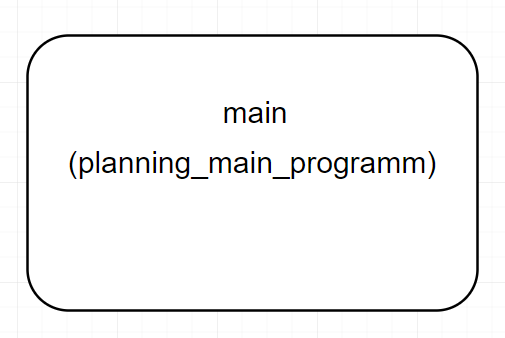
\includegraphics[width=0.4\textwidth]
        {img/diag_planning_main_programm.png}
        \caption{} Architektur der Quellcode-Datei main.lisp}
\end{figure}



\subsection{Beschreibung des Teilsystems}
\subsubsection{\"Ubersicht}
\chapterauthor{Kevin Störmer}
Die Quellcode-Datei 'main' im Paket 'planning\_main\_programm' soll ausschliesslich auf höchster Ebene den internen Ablauf des PR2 modellieren. 

Alle dafür notwendigen Logiken, die auf Basis externer Daten entschieden werden, wurden dabei basierend auf der Quelle der Daten in andere Quellcode-Dateien ausgelagert. Dabei wurde z.b der Vergleich zweier Punkte aus Vision in die Quellcode-Datei 'vision-communicate' (Paket: planning\_vision) ausgelagert.




\subsubsection{main ()}
\chapterauthor{Vanessa Hassouna}
\begin{verbatim}
main()
Die Main startet eine 'ros-node' mit dem Namen \textit{planning\_main}.
Diese Node läuft solange,bis die komplette Main einmalig durchlaufen wurde. 
@return: T oder Nil 
\end{verbatim}



\subsection{Programmablauf}
\chapterauthor{Vanessa Hassouna}
\subsubsection{Schritt 1: Vorbereiten des Roboters}
Der Pr2 begibt sich in die Homeposition, von der aus er Objekte sehen soll. 

\subsubsection{Schritt 2: Suche nach Objekten}
Jedes Mal, wenn der Kopf des Pr2 sich in einer bestimmten Position befindet, wird der Service \textit{/vision\_suturo/objects\_information} aufgerufen. Die gegebenen Information werden wie folgt bearbeitet:

\begin{itemize}
\item Die gegebenen Informationen werden extrahiert.
\item Die beiden Arrays \textbf{normal\_features} und \textbf{color\_features} werden zergliedert und mit Hilfe von \textbf{object\_amount} identifiziert und auf dem "Param-Server" gespeichert.
\item Die normal\_features und color\_features werden konkateniert auf dem "Param-Server" als \textbf{featuresX} gespeichert, wobei X hier die Nummer des Objektes darstellt.
\item Die \textbf{object\_pose} wird als Array global gespeichert.
\end{itemize}



\subsubsection{Schritt 3: Weitergabe} 

\begin{itemize} 
\item Jetzt werden die gesehenen Objekte an Knowledge weitergegeben, hier bekommen wir für jedes gegebene Objekt ein Label als String zurück.
\item Mit Hilfe des erhaltenen Labels rufen wir den Service '/vision\_suturo/objects\_pose' von Vision auf, der anhand von Objekt-Nummer und Label uns eine Pose zurück gibt.  
\item Wenn die Pose bei uns angekommen ist, publishen wir auf ein Topic von Knowledge, damit das gesehene Objekt in der Wissensbasis gespeichert wird.
\end{itemize}





\subsubsection{Schritt 4: Welches Objekt soll ich greifen und wo soll es hin}
Wir erfragen bei Knowledge welche Objekte wir greifen sollen, in dem wir den Service "knowledge\_msgs/ObjectsToPick" \\
aufrufen. Als Antwort bekommen wir 2 Strings zurück.
Mit der Funktion calculate-landing-zone-visualized() erhalten wir dann einen Standpunkt wohin das Objekt platziert werden soll. %X=HAUKES FUNKTION
Des Weiteren wird noch abgefragt wie das Objekt gegriffen werden soll. Diese Information wird dann weiter an Motion gegeben.

\subsubsection{Schritt 5: Hinfahren zum gegebenen Ort}
Mit Hilfe des Punktes wird berechnet wo der Roboter hinfahren muss. 
 
\subsubsection{Schritt 6: Abstellen und weiter}
Das Objekt wird abgestellt.
Danach fährt der Pr2 wieder zu seiner Homeposition und sucht die nächsten Objekte.






\subsubsection{find-Object(x z)}
\chapterauthor{Kevin Störmer}
\begin{verbatim}
find-Object()
Beschreibung: Sucht anhand variabler x und z-Achse sowie fest eingestellter
y-Koordinaten nach sichtbaren Objekten. Sollte ein Objekt gefunden werden,
oder die maximale Anzahl an Suchläufen überschritten werden,
terminiert die Funktion. Die Funktion beginnt immer beim zuletzt gesehenen Punkt.
@param: x-axis z-axis
@return: T wenn Objekt gefunden, nil falls nichts zu finden
\end{verbatim}




\newpage
\section{Die Quellcode-Datei: vision\_communicate.lisp (planning\_vision)}

\subsection{Architekturbild}

\chapterauthor{Vanessa Hassouna}



\begin{figure}[!htb]
        \center{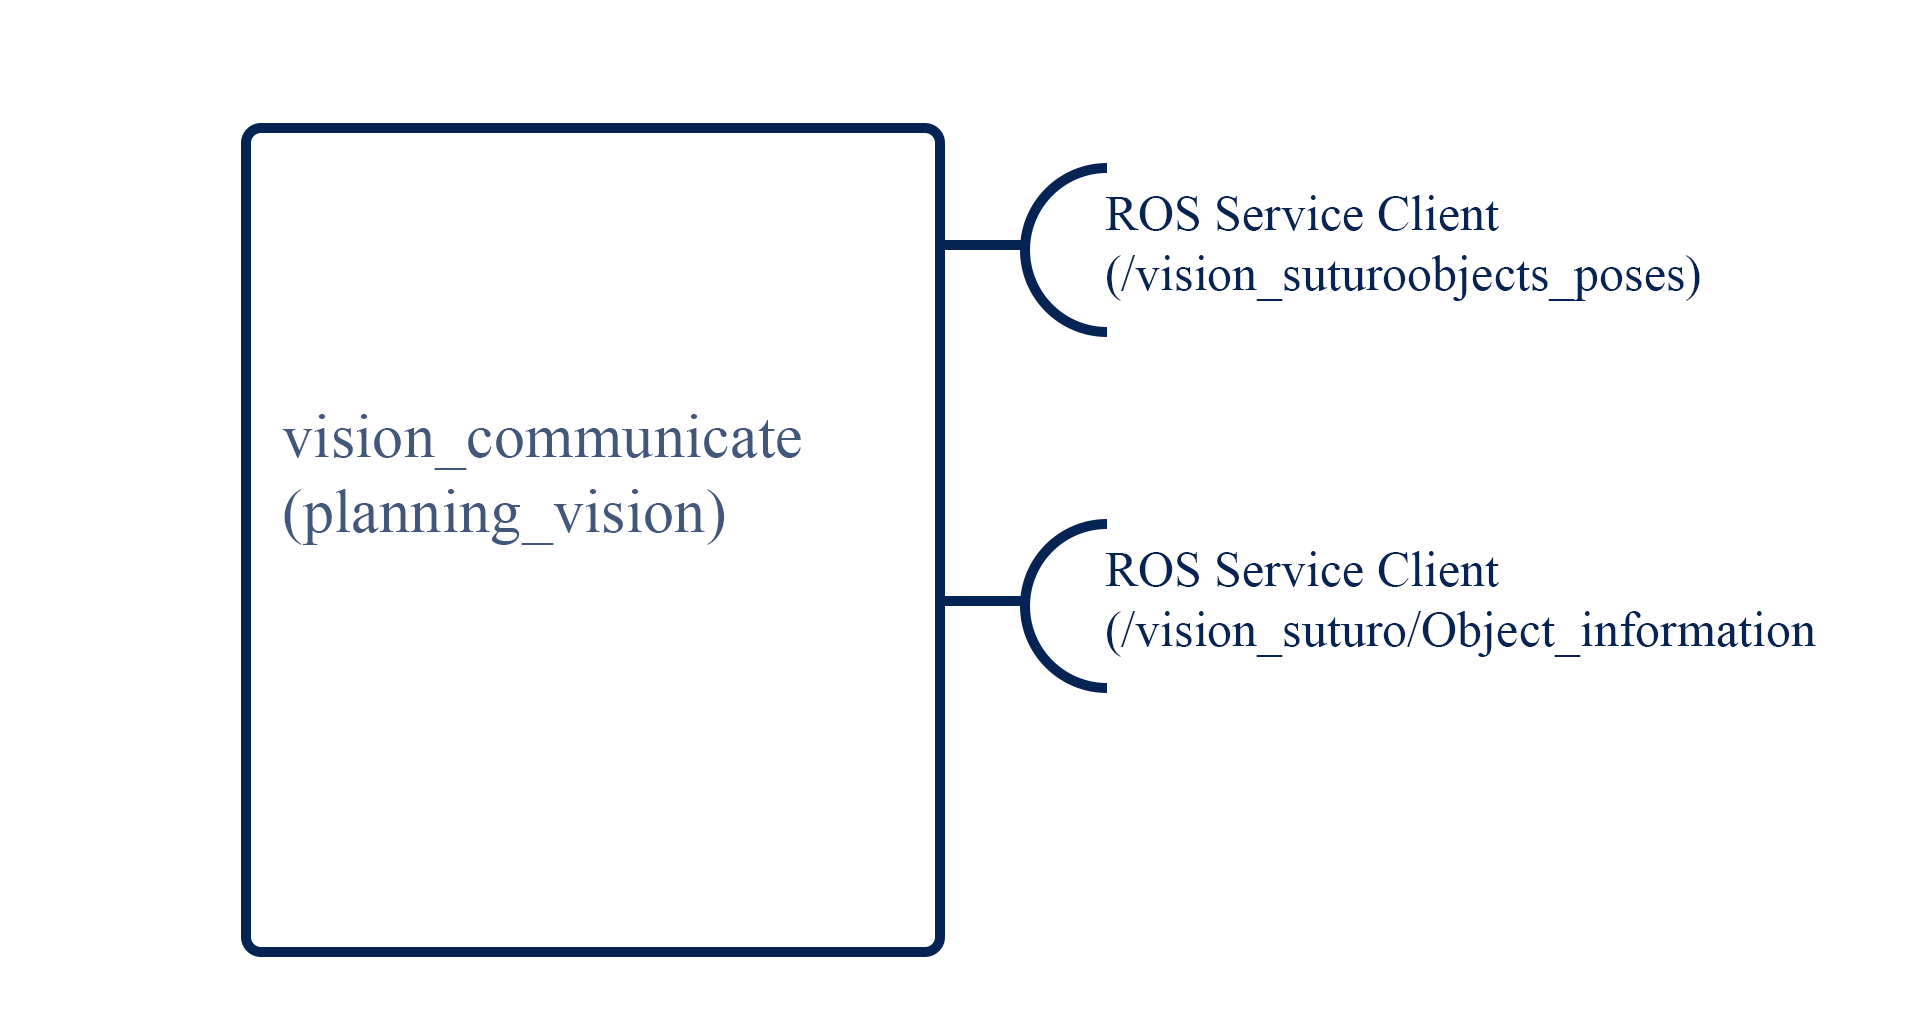
\includegraphics[width=0.6\textwidth]
        {img/vision.png}
        \caption{} Architektur der Quellcode-Datei vision\_communicate.lisp}
\end{figure}




\subsection{API}
\chapterauthor{Vanessa Hassouna}
\subsubsection{Serviceclients}
1. '/vision\_suturo/Object\_information' \\
Nimmt Objekt über Kinect wahr und gibt eine 'msg' zurück mit Informationen.\\ \\
2. '/vision\_suturo/objects\_pose' \\
Gibt zu einem Objekt (übergeben als Nummer) und einem Label (übergeben als String) die Pose mit Rotation zurück.

\subsection{Beschreibung des Teilsystems}




\subsubsection{call-Vision-Object-Clouds ()}
\chapterauthor{Vanessa Hassouna}
\begin{verbatim}
call-Vision-Object-Clouds ()

Beschreibung: Der Service von Vision "/vision\_suturo/objects\_information"
wird aufgerufen.

@return: Successfull oder Aborted
\end{verbatim}


\subsubsection{check-Points-Is-Equal (msg-one msg-two delta))}
\chapterauthor{Kevin Störmer}
\begin{verbatim}
check-Points-Is-Equal (msg-one msg-two delta)

Beschreibung: Vergleicht 2 object_detection-srv:object in
ihren x, y, z Koordinaten anhand eines übergebenen Deltas.
Überschreitet die Differenz der beiden Messages das Delta
wird nil zurückgegeben.

@param: object_detection-srv:object msg-one 
object_detection-srv:object msg-two int delta
@return: T or nil
\end{verbatim}

\section{Die Quellcode-Datei: knowledge-communicate.lisp\\
planning\_knowledge)}

\subsection{Architekturbild}
\chapterauthor{Vanessa Hassouna}

\begin{figure}[!htb]
        \center{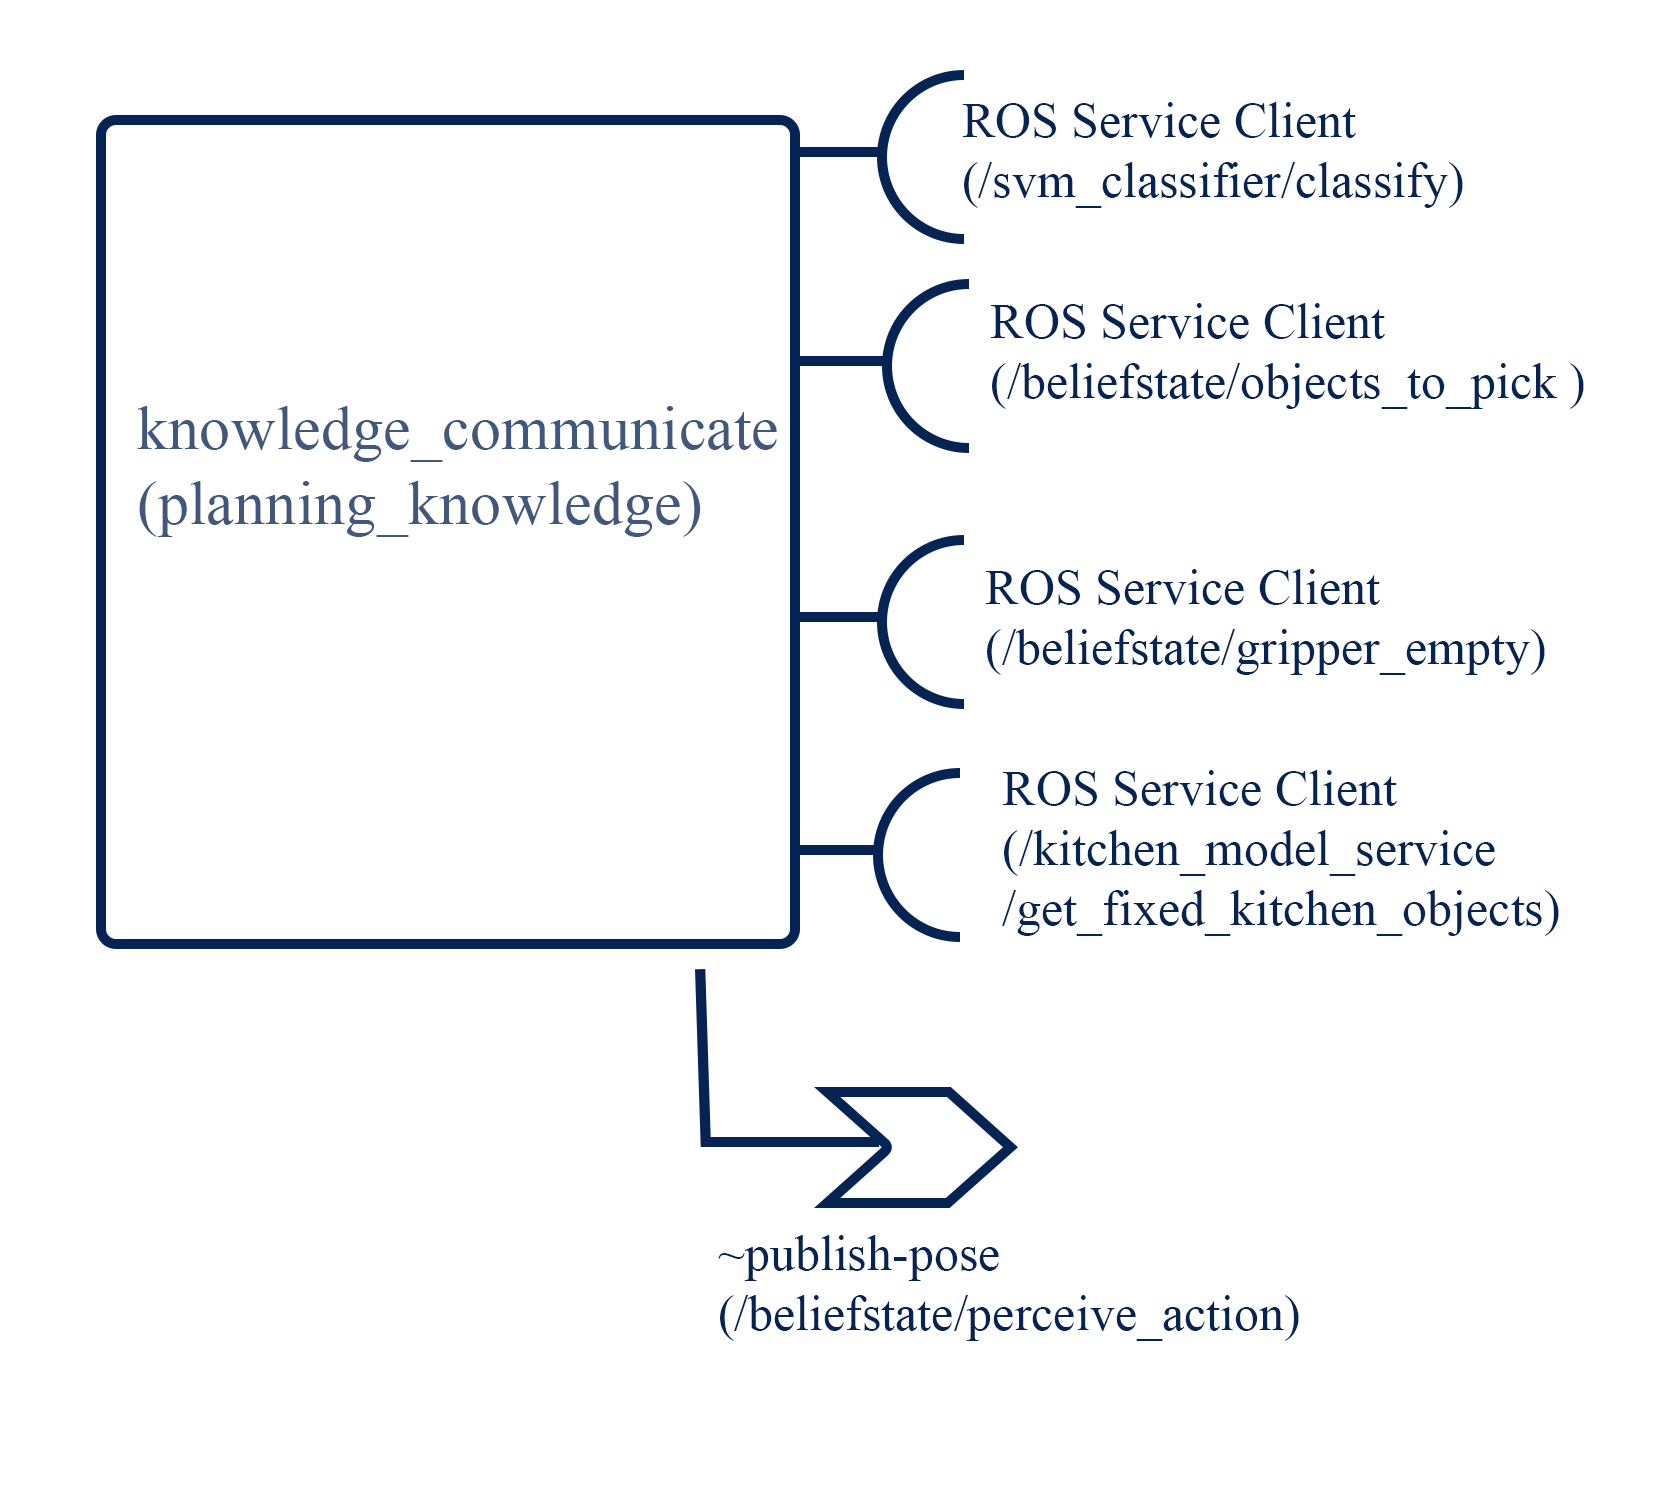
\includegraphics[width=0.6\textwidth]
        {img/knowledge.png}
        \caption{} Architektur der Quellcode-Datei knowledge-communicate.lisp}
\end{figure}

\subsection{API}
\chapterauthor{Vanessa Hassouna}
\subsubsection{Serviceclients}
1. 'svm\_classifier/classify' \\
Gibt uns ein Label als String für ein Objekt zurück.\\

2. 'beliefstate/objects\_to\_pick'\\
Gibt uns zwei Strings zurück. Diese sind leer, wenn kein Objekt mehr gegriffen werden soll oder es kein Objekt mehr zum Greifen gibt.

3. 'beliefstate/gripper\_empty'\\
Wir können erfragen, welcher Gripper frei ist.\\

4. 'kitchen\_mode\_service/get\_fixed\_kitchen\_objects'\\
%?
\subsubsection{Topics}
1. 'beliefstate/perceive\_action'\\
Wenn ein Objekt wahrgenommen wurde, publishen wir diese Information.


\subsection{Beschreibung des Teilsystems}
\subsubsection{\"Ubersicht}
\chapterauthor{Kevin Störmer}
Die Quellcode-Datei 'knowledge-communicate' im Paket 'planning\_knowledge' ist ausschliesslich für die Kommunikation mit Modulen der Gruppe Knowledge zust\"andig.



%%%%%%%%%%%%%%%%%%%%%%%%%%%%%%%%%%%%%%%%%%%%%%%%%%%%%%%%%%%%%%%%%%%%%%%%%%%%%%

\section{Die Quellcode-Datei: motion-actions.lisp (planning\_motion)}
\subsection{Architekturbild}
\chapterauthor{Vanessa Hassouna}


\begin{figure}[!htb]
        \center{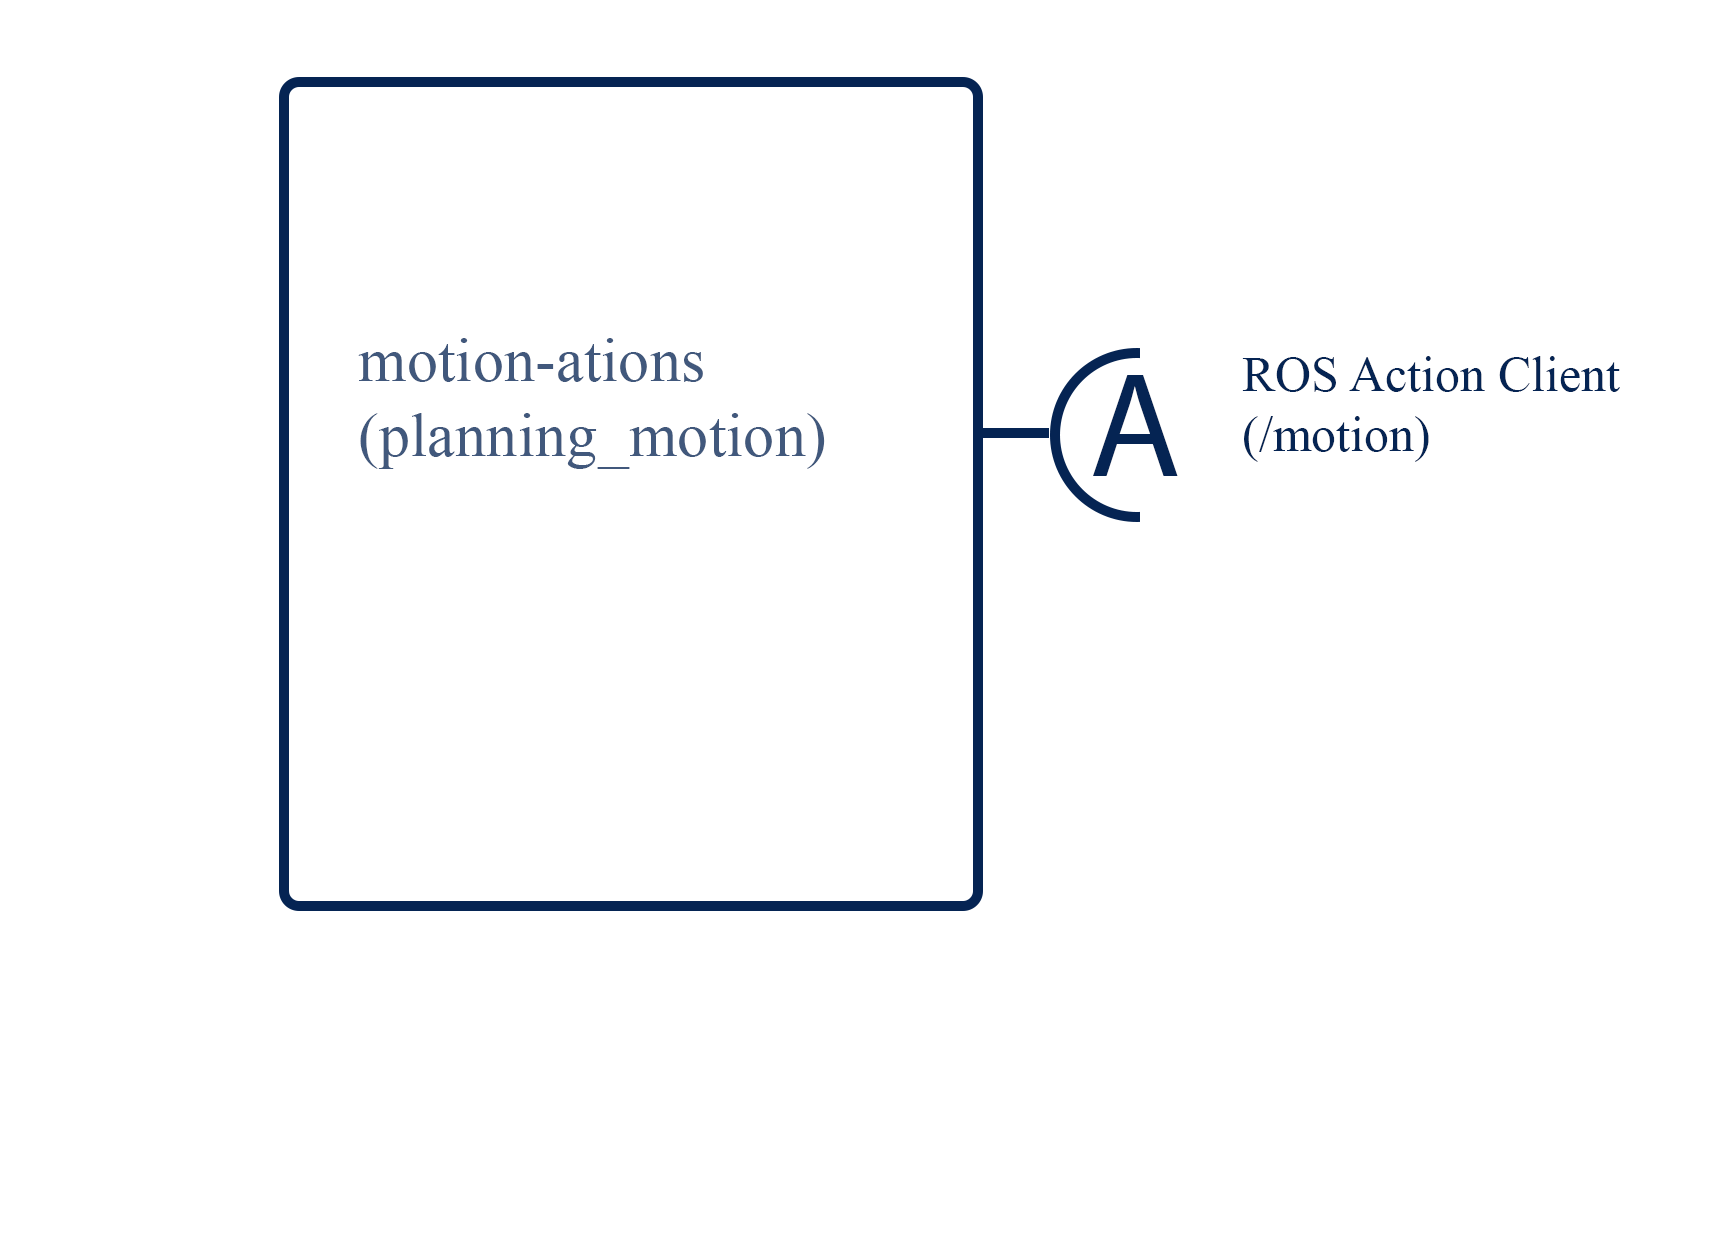
\includegraphics[width=0.6\textwidth]
        {img/motion.png}
        \caption{} Architektur der Quellcode-Datei motion-actions.lisp}
\end{figure}




\subsection{API}
\chapterauthor{Kevin Störmer}
\subsubsection{Actionclients}
1. '/motion' \\
Bewegt die Arme des Pr2 entweder in die Home-Position oder zu einem bestimmten Punkt.
\subsection{Beschreibung des Teilsystems}
\subsubsection{\"Ubersicht}
\chapterauthor{Kevin Störmer}
Die Quellcode-Datei 'motion-actions' im Paket 'planning\_motion'  ist ausschliesslich für die Kommunikation mit Modulen der Gruppe Motion zuständig. Dabei wird die Action '/motion' einmal für die Home-Position des Pr2, zum Bewegen des Armes zu einem bestimmten Punkt und zum Greifen genutzt.


\subsubsection{call-Motion-\\
Move-Arm-Homeposition()}
\chapterauthor{Vanessa Hassouna und Hauke Tietjen}
\begin{verbatim}
call-Motion-Move-Arm-Homeposition()

Beschreibung: Ruft den Actionserver von Motion auf und
sendet das 'Command 2'.Dieses Command lässt die Arme des Pr2 
in die Homeposition fahren.

@return: Successfull oder Aborted
\end{verbatim}



\subsubsection{call-Motion-\\
Move-Arm-To-Point (point-center-\\of-object \&optional (x 3))
}
\chapterauthor{Vanessa Hassouna und Hauke Tietjen}
\begin{verbatim}
call-Motion-Move-Arm-To-Point (point-center-of-object \&optional (x 3))

Beschreibung: Ruft den Actionserver von Motion auf und 
sendet den Befehl einen Arm zu dem point-center-of-object zu fahren.
@param point-center-of-object &optional (x 3)
@return: Successfull oder Aborted
\end{verbatim}

\newpage
\section{Die Quellcode-Datei: movement.lisp (planning\_move)}
\subsection{Architekturbild}
\chapterauthor{Kevin Störmer}


\begin{figure}[!htb]
        \center{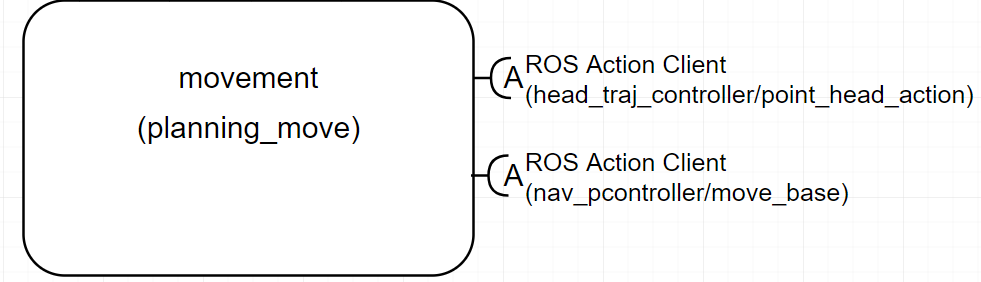
\includegraphics[width=0.8\textwidth]
        {img/diag_planning_move.png}
        \caption{} Architektur der Quellcode-Datei movement.lisp}
\end{figure}


\subsection{API}
\chapterauthor{Kevin Störmer}
\subsubsection{Actionclients}
1. 'head\_traj\_controller/point\_head\_action' \\
Bewegt den Kopf des Pr2 in Richtung eines Punktes.\\ \\
2. 'nav\_pcontroller/move\_base' \\
Bewegt die Basis des Pr2 in Richtung eines Punktes.
\subsection{Beschreibung des Teilsystems}

\subsubsection{\"Ubersicht}
\chapterauthor{Kevin Störmer}
Die Quellcode-Datei actions.lisp im Paket 'planning\_motion'  ist ausschliesslich für die Kommunikation mit Gruppe Motion zuständig. Dabei wird die Action '/motion' einmal für die Home-Position des Pr2 und zum Bewegen des Armes zu einem bestimmten Punkt genutzt.



\subsubsection{move-head (x y z)}
\chapterauthor{Kevin Störmer}

\begin{verbatim}
move-Head (x y z)
Beschreibung: Lässt den Rr2-Kopf bewegen, dabei wird der Service 
"head\_traj\_controller/point\_head\_action" angesprochen.
x,y, und z werden als Koordinaten ausgehend von base_link behandelt.
@param: x y z
@return: Succesfull oder Aborted
\end{verbatim}


\subsubsection{move-Base-To-\\
Point-Safe (x y z angle))
}
\chapterauthor{Vanessa Hassouna}
\begin{verbatim}
move-Base-To-Point-Safe (x y z angle)

Beschreibung: Diese Methode lässt den Roboter an eine vordefinierte 
Position fahren, bei der er sich ungehindert drehen kannn.
Danach fährt der Pr2 zu dem gewünschten Punkt.
@param: x y z angle
@return: Successfull oder Aborted
\end{verbatim}


\subsubsection{move-Base-To-\\
Point (x y z angle)}
\chapterauthor{Vanessa Hassouna}
\begin{verbatim}
move-Base-To-Point (x y z angle)

Beschreibung: Anhand des Actionservice "nav\_pcontroller/move\_base" 
wird die Basis bewegt. Der Punkt und die Rotation sind in Frame "map" anzugeben.

@param: x y z angle
@return: Successfull oder Aborted
\end{verbatim}


\subsubsection{move-Robo-Into\\
-Homeposition ()}
\chapterauthor{Vanessa Hassouna}
\begin{verbatim}
move-Robo-Into-Homeposition ()

Beschreibung: move-Base-To-Point wird aufgerufen mit 
von uns vordefinierten Punkten, die als Homeposition dienen.

@return: Succesfull oder Aborted
\end{verbatim}


\subsubsection{init-Robo-Moving ()}
\chapterauthor{Vanessa Hassouna}
\begin{verbatim}
init-Robo-Moving ()

Beschreibung: Diese Hilfsfunktion dient dazu,
die Initialisierung für das Fahren in der Simulation zu übernehmen.

@return: Successfull oder Aborted
\end{verbatim}

\subsubsection{init-Action-Client-Base ()}
\chapterauthor{Vanessa Hassouna}
\begin{verbatim}
init-Action-Client-Base ()

Beschreibung: Diese Hilfsfunktion dient dazu, 
den Action-Client zu initialisieren.

@return: Successfull oder Aborted
\end{verbatim}

\subsubsection{get-Action-Client-Base ()}
\chapterauthor{Vanessa Hassouna}
\begin{verbatim}
get-Action-Client-Base ()

Beschreibung: Diese Hilfsfunktion dient dazu, den Action-Client zu erhalten.

@return: Successfull oder Aborted
\end{verbatim}






\section{Die Quellcode-Datei: external-logic.lisp (planning\_logic)}
\subsection{Architekturbild}
\chapterauthor{Vanessa Hassouna}


\begin{figure}[!htb]
        \center{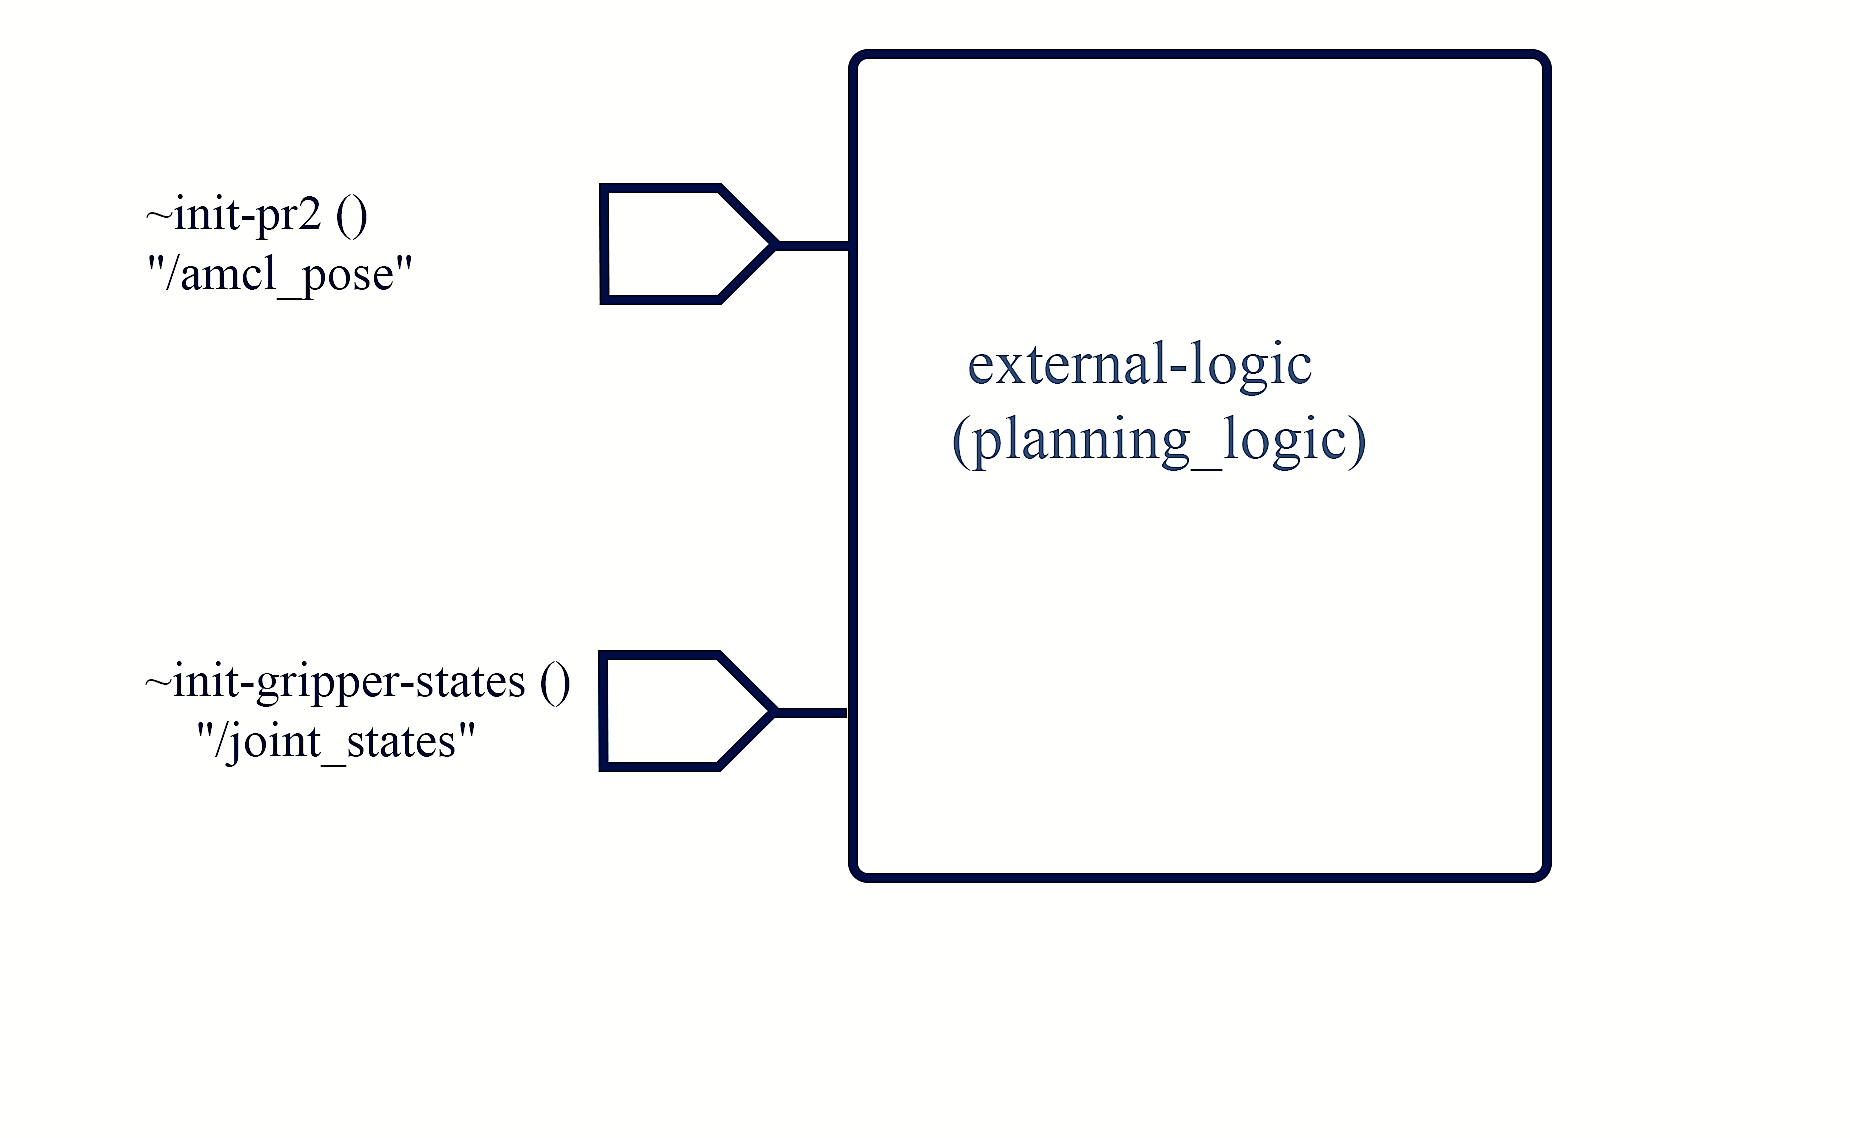
\includegraphics[width=0.8\textwidth]
        {img/externallogic.png}
        \caption{} Architektur der Quellcode-Datei movement.lisp}
\end{figure}


\subsection{API}
\chapterauthor{Vanessa Hassouna}
\subsubsection{Topics}
1. 'joint\_states' \\
Subscribed das Topic und speichert die Werte des Grippers.\\
 %vielleicht willst du hier was schreiben?
 
2. 'robot\_pose' \\
Subscribed das Topic und gibt uns die Position des Roboters.
\subsection{Beschreibung des Teilsystems}

\subsubsection{\"Ubersicht}
\chapterauthor{Vanessa Hassouna}
Die Quellcode-Datei 'external-logic.lisp' im Paket 'planning\_logic' ist für reine logische Funktionen vorgesehen.



\subsubsection{transformation-Vision-Point (pose amount\\
\&optional (endFrame '/base\_footprint')}
\chapterauthor{Vanessa Hassouna}
\begin{verbatim}
transformation-Vision-Point (pose amount &optional (endFrame "/base\_footprint")

Beschreibung: Das gegebene Objekt wird von dem ausgehenden Frame
in ein optionales Frame umgewandelt.

@param: pose, amount und optional endFrame
@return: Liefert eine transformierte tf-point-stamped
\end{verbatim}




\subsubsection{catch-Transformation \\
(transform-listener tf-point-stamped endFrame)}
\chapterauthor{Vanessa Hassouna}
\begin{verbatim}
catch-Transformation (transform-listener tf-point-stamped endFrame)

Beschreibung: Hier findet die eigentliche Transformation statt.

@param: transform-listener tf-point-stamped endFrame
@return: Liefert eine transformierte tf-point-stamped
\end{verbatim}


%KOMMT NOCH(defun let-Robo-Try-To-Poke (point-for-motion number-for-arm)
%KOMMT NOCH (defun try-To-Poke-Different-Location(point-for-motion number-for-arm)


\subsubsection{should-Robo-Use-Left-Or-Right-Arm(pose amount \\
\&optional (endFrame '/base\_footprint'))}
\chapterauthor{Vanessa Hassouna}
\begin{verbatim}
should-Robo-Use-Left-Or-Right-Arm (pose amount &optional
(endFrame "/base\_footprint"))

Beschreibung: Anhand der Y-Achse entscheidet der Roboter
ob er den linken oder rechten Arm bewegen soll.

@param: pose object-number &optional endFrame
@return: 3 oder 2 (3 = links 2 = Rechts)
\end{verbatim}


\subsubsection{disassemble-Vision-Call (visionclouds)}
\chapterauthor{Vanessa Hassouna}
\begin{verbatim}
disassemble-Vision-Call (visionclouds)

Beschreibung: Extrahiert alle Informationen aus der 
Visioncloud und speichert normal\_features, color\_features, 
object\_amount und object\_pose auf den Param-Server.
 
@param: visionclouds
@return: object\_pose
\end{verbatim}



\subsubsection{set-Params-Features \\
(normal-s color-s normal-e color-e amount)}
\chapterauthor{Vanessa Hassouna}
\begin{verbatim}
set-Params-Features (normal-s color-s normal-e color-e amount)

Beschreibung: Eine Hilfsfunktion für die Funktion "disassemble-Vision-Call", 
um aus normal\_features und color\_features konkateniert ein features-X zu 
erstellen. (Knowledge benötigt ein Array in dem zuerst color\_features 
vorkommen und direkt im Anschluss normal_features)

@param: normal-s color-s normal-e color-e amount
@return: Nil
\end{verbatim}


\subsubsection{init-pr2()}
\chapterauthor{Vanessa Hassouna}
\begin{verbatim}
init-pr2 ()

Beschreibung: Subscribed das Topic '/amcl_status'.

@return: geometry_msgs/Pose
\end{verbatim}

\subsubsection{pose-cb (msg)}
\chapterauthor{Vanessa Hassouna}
\begin{verbatim}
pose-cb (msg)

Beschreibung: Callback-Funktion für "init-pr2" die durchgängig die Fluents
*pr2-pose* aktualisiert.

@param: msg
@return: geometry_msgs/Pose
\end{verbatim}

\subsubsection{move-pr2 (x y z)}
\chapterauthor{Vanessa Hassouna}
\begin{verbatim}
move-pr2 (x y z)

Beschreibung: Ruft move-Base-To-Point-Safe mit angle-From-Pr2-Pose-To-Point auf.

@param: x y z 
@return: Successfull oder Aborted
\end{verbatim}

\subsubsection{angle-From-Pr2-Pose-To-Point (x-goal y-goal z-goal)}
\chapterauthor{Vanessa Hassouna}
\begin{verbatim}
angle-From-Pr2-Pose-To-Point (x-goal y-goal z-goal)

Beschreibung: Berechnet von der aktuellen Position des Roboters um wie viel Grad
er sich drehen muss, damit er zu einem Punkt fahren kann. Dafür wurde unter 
anderem das Paket "Cram-Language" mit der Funktion 'atan' benutzt. 
Da das Bewegen des Pr2 in dem Frame "\map" stattfindet, wurde hier zusätzlich 
noch die aktuelle Drehung in der Welt gespeichert. Dies wird dann mit dem 
Grad, um wie viel der Pr2 sich drehen muss, gegengerechnet, 
so dass am Ende ein Winkel produziert wird, der innerhalb des Frames "\map" funktioniert.

@param: x-goal y-goal z-goal 
@return: angle 
\end{verbatim}


\subsubsection{try-To-Poke-Different-Location\\
(point-for-motion number-for-arm)}
\chapterauthor{Vanessa Hassouna}
\begin{verbatim}
try-To-Poke-Different-Location\\
(point-for-motion number-for-arm)

Beschreibung: Die Funktion lässt den Roboter 
anhand vorgegebener Positionen seine Drehung sowie seine
Position ändern, wenn er ein Objekt nicht erreichen kann.

@param: point-for-motion number-for-arm
@return: T oder Nil


\end{verbatim}


\subsubsection{init-gripper-states ()}
\chapterauthor{Kevin Störmer}
\begin{verbatim}
init-gripper-states ()
Beschreibung: Subscribed das Topic '/joint_states' und gibt als Callback-Funktion
'is-gripper-filled (msg)' an.
\end{verbatim}

\subsubsection{is-gripper-filled (msg)}
\chapterauthor{Kevin Störmer}
\begin{verbatim}
is-gripper-filled (msg)
Beschreibung: Aktualisiert alle 0.01 Sekunden die Fluents *gripper-righ-state-fluent* 
und *gripper-left-state-fluent* um T oder nil. Dabei wird anhand der Joint-States der
Gripper-Joints 'r_gripper_joint' und 'l_gripper_joint' entschieden
ob jeder Gripper des Pr2 gefüllt ist, oder nicht. Diese werte werden
aus den Joint-States geparsed.
@param: sensor_msgs/JointState msg 
\end{verbatim}



\section{Die Quellcode-Datei: objects.lisp (planning\_objects)}
\subsection{Architekturbild}
\chapterauthor{Hauke Tietjen}



\begin{figure}[!htb]
	\center{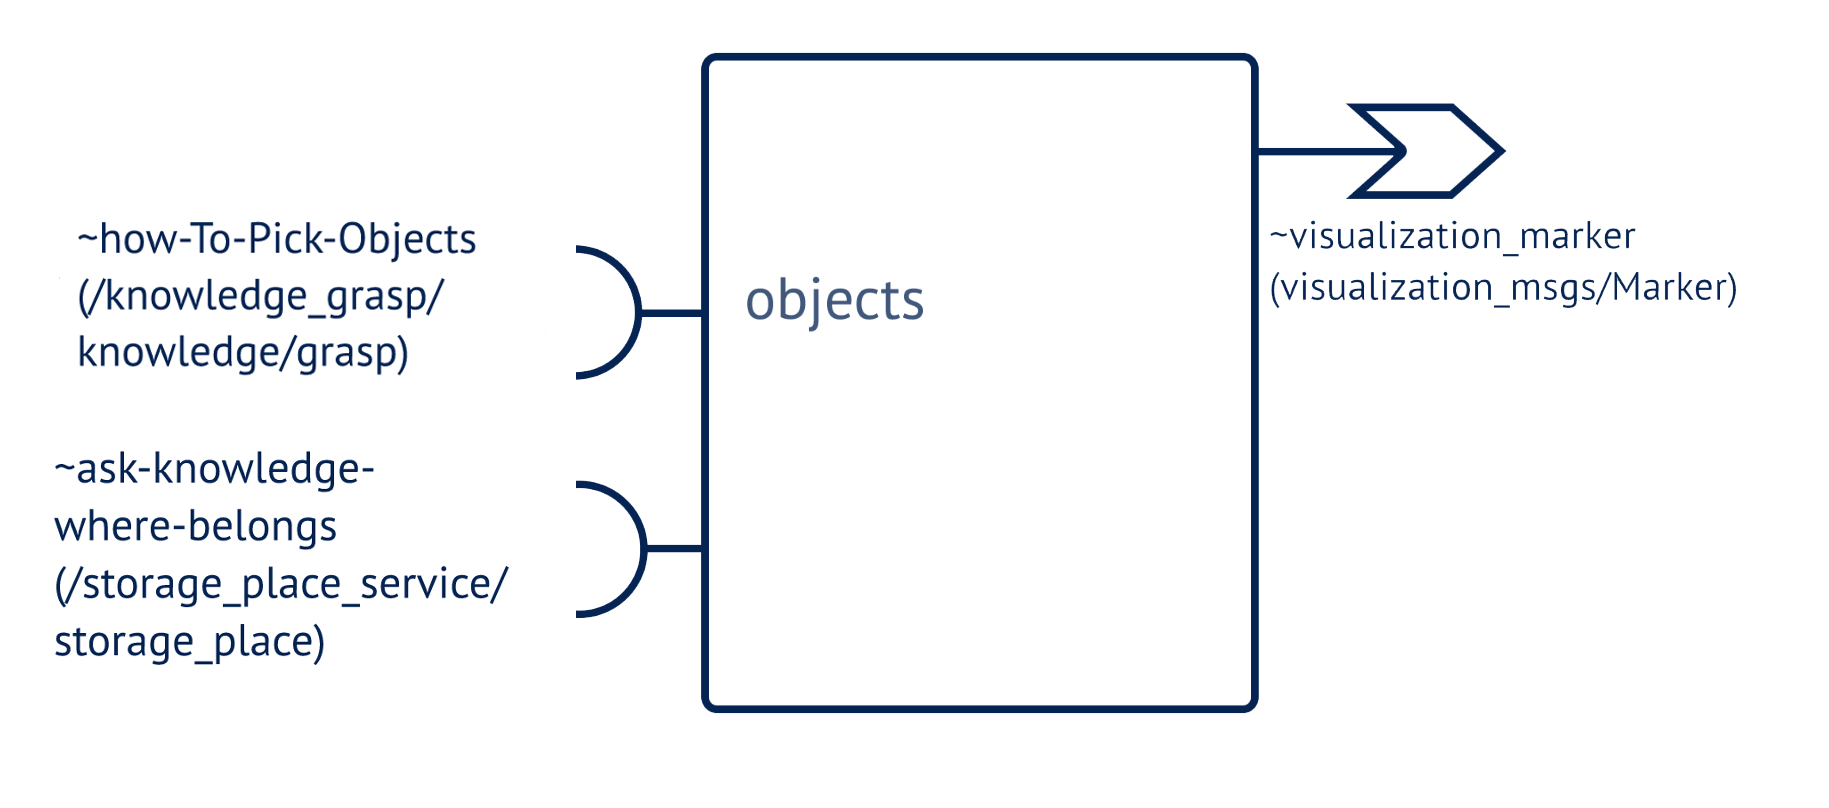
\includegraphics[width=1.0\textwidth]
		{img/diag_planning_objects.png}
		\caption{} Architektur der Quellcode-Datei planning-objects.lisp}
\end{figure}


\subsection{API}
\chapterauthor{Hauke Tietjen}
\subsubsection{Serviceclients}
1. '/storage\_place\_service/storage\_place' \\
Gibt den Ablageplatz des Objekts zur\"uck.\\ \\
2. '/object\_grasping/grasp\_pose' \\
Gibt die Greifpose des für die Koordinaten zurück.\\
3. '~location\_marker' \\
Publiziert Marker zur Visualisierung von Landezonen.
\subsection{Beschreibung des Teilsystems}
\subsubsection{\"Ubersicht}
\chapterauthor{Hauke Tietjen}
Die Datei 'objects' aus dem Paket 'planning\_objects' dient dazu aus den von Knowledge vorgegebenen Ablageorten für Objekte Punkte zu bestimmen die geeignet sind um Objekte auf ihnen abzustellen. Dabei werden Platzmangel, Kollision und das Herunterfallen von Objekten berücksichtigt. Zusätzlich lassen sich die finalen Positionen in Rviz visualisieren.

\subsubsection{calculate-landing-zone()}
\chapterauthor{Hauke Tietjen}
\begin{verbatim}
calculate-landing-zone()
Beschreibung: Fragt Knowledge an welchen Ablageort das Objekt gehört und
verkleinert ihn um das Herunterfallen der Objekte von Tischkanten zu
verhindern. Ruft danach fill-landing-zone-horizontally auf das eine Pose zurück gibt.
@param object
@return Gibt eine Pose in /map zurück um ein Objekt zu greifen
\end{verbatim}

\subsubsection{fill-landing-zone-horizontally()}
\chapterauthor{Hauke Tietjen}
\begin{verbatim}
fill-landing-zone-horizontally()
Beschreibung: Befüllt den Ablageort mit einem Objekt pro Aufruf, von Links nach
Rechts auf der Y-Achse im Frame /map. Fragt Knowledge nach der Z-Achse und Pose
wo das Objekt gegriffen werden soll.
@param position width height
@return Gibt eine Pose in /map zurück um ein Objekt zu greifen
\end{verbatim}

\subsubsection{calculate-landing-zone-visualized()}
\chapterauthor{Hauke Tietjen}
\begin{verbatim}
calculate-landing-zone-visualized()
Beschreibung: Führt calculate-landing-zone() aus und visualisiert das Ergebnis mit
visualize-landing-zone().
@param object
@return Gibt eine Pose in /map zurück um ein Objekt zu greifen
\end{verbatim}

\subsubsection{visualize-landing-zone()}
\chapterauthor{Hauke Tietjen}
\begin{verbatim}
visualize-landing-zone()
Beschreibung: Führt vis-init() und publish-pose() aus um eine Pose zu visualisieren.
@param pose
@return 
\end{verbatim}

\subsubsection{check-which-storage-place()}
\chapterauthor{Hauke Tietjen}
\begin{verbatim}
check-which-storage-place()
Beschreibung: Findet heraus in welchem der vier Storageplaces sich die Y-Koordinate befindet.
@param y
@return Storageplace
\end{verbatim}

\subsubsection{vis-init()}
\chapterauthor{Hauke Tietjen}
\begin{verbatim}
vis-init()
Beschreibung: Startet den Marker-publisher.
@param 
@return 
\end{verbatim}

\subsubsection{publish-pose()}
\chapterauthor{Hauke Tietjen}
\begin{verbatim}
publish-pose
Beschreibung: Publiziert einen Marker mit ID an der angegebenen Pose mit den Dimensionen
aus height und width.
@param pose id height width
@return 
\end{verbatim}

\section{Die Quellcode-Datei: error-hierarchy.lisp (planning\_error)}
\subsection{Architekturbild}
\chapterauthor{Hauke Tietjen}
\begin{figure}[!htb]
	\center{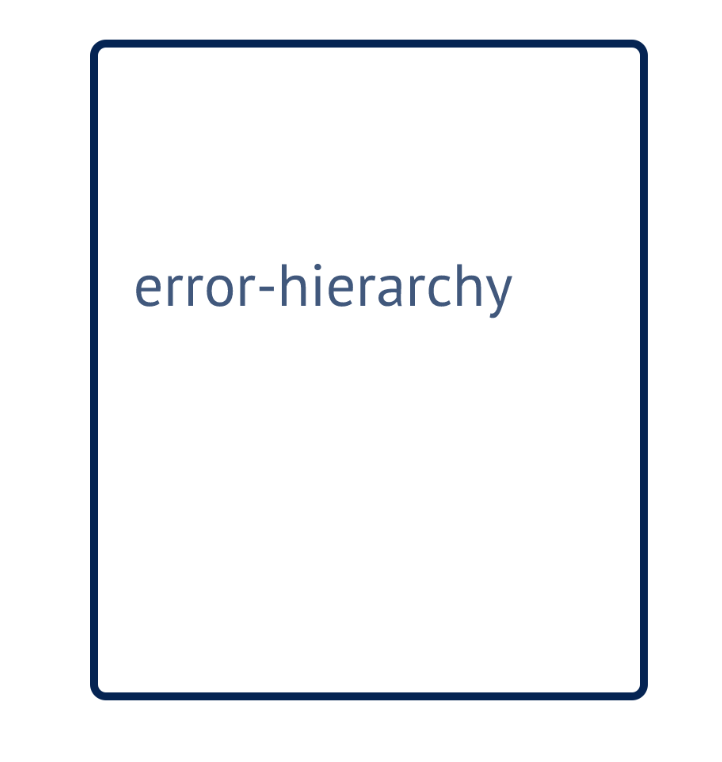
\includegraphics[width=0.4\textwidth]
		{img/diag_planning_error.png}
		\caption{} Architektur der Quellcode-Datei error-hierarchy.lisp}
\end{figure}


\subsection{API}
\chapterauthor{Hauke Tietjen}
\subsubsection{Serviceclients}
keine
\subsection{Beschreibung des Teilsystems}
\subsubsection{\"Ubersicht}
\chapterauthor{Hauke Tietjen}
Die Datei 'error-hierarchy' aus dem Paket 'planning\_error' legt die Hierarchie der Fehler fest.

\subsubsection{custom-error()}
\chapterauthor{Hauke Tietjen}
\begin{verbatim}
custom-error()
Beschreibung: Dieser Standardfehler erbt von 'error' während alle weiteren Fehler von diesem erben. 
@param message
@return 
\end{verbatim}

\subsubsection{vision-error()}
\chapterauthor{Hauke Tietjen}
\begin{verbatim}
vision-error()
Beschreibung: Ein Fehler bei dem es um etwas aus dem Bereich Vision geht kann hiermit
beschrieben werden. Vor der Fehlernachricht wird jetzt 'vison error:' ausgegeben. 
@param
@return 
\end{verbatim}

Die Conditions 'motion-error', 'move-error', 'knowledge-error' und 'objects-error' sind analog zu 'vison-error' und definieren einfach weitere Fehler für andere Bereiche.


\newpage
\section*{Methodendokumentation Gruppe Knowledge}
\section{knowledge\_grasp}
\chapterauthor{Max-Phillip Bahr}
Das Knowledge\_Grasp-Paket dient dazu die GraspPose zu einem erkannten Gegenstand aus der Ontologie auszulesen, an der der PR2 diesen Gegenstand vor ihm greifen soll.

\begin{figure}[!htb]
        \center{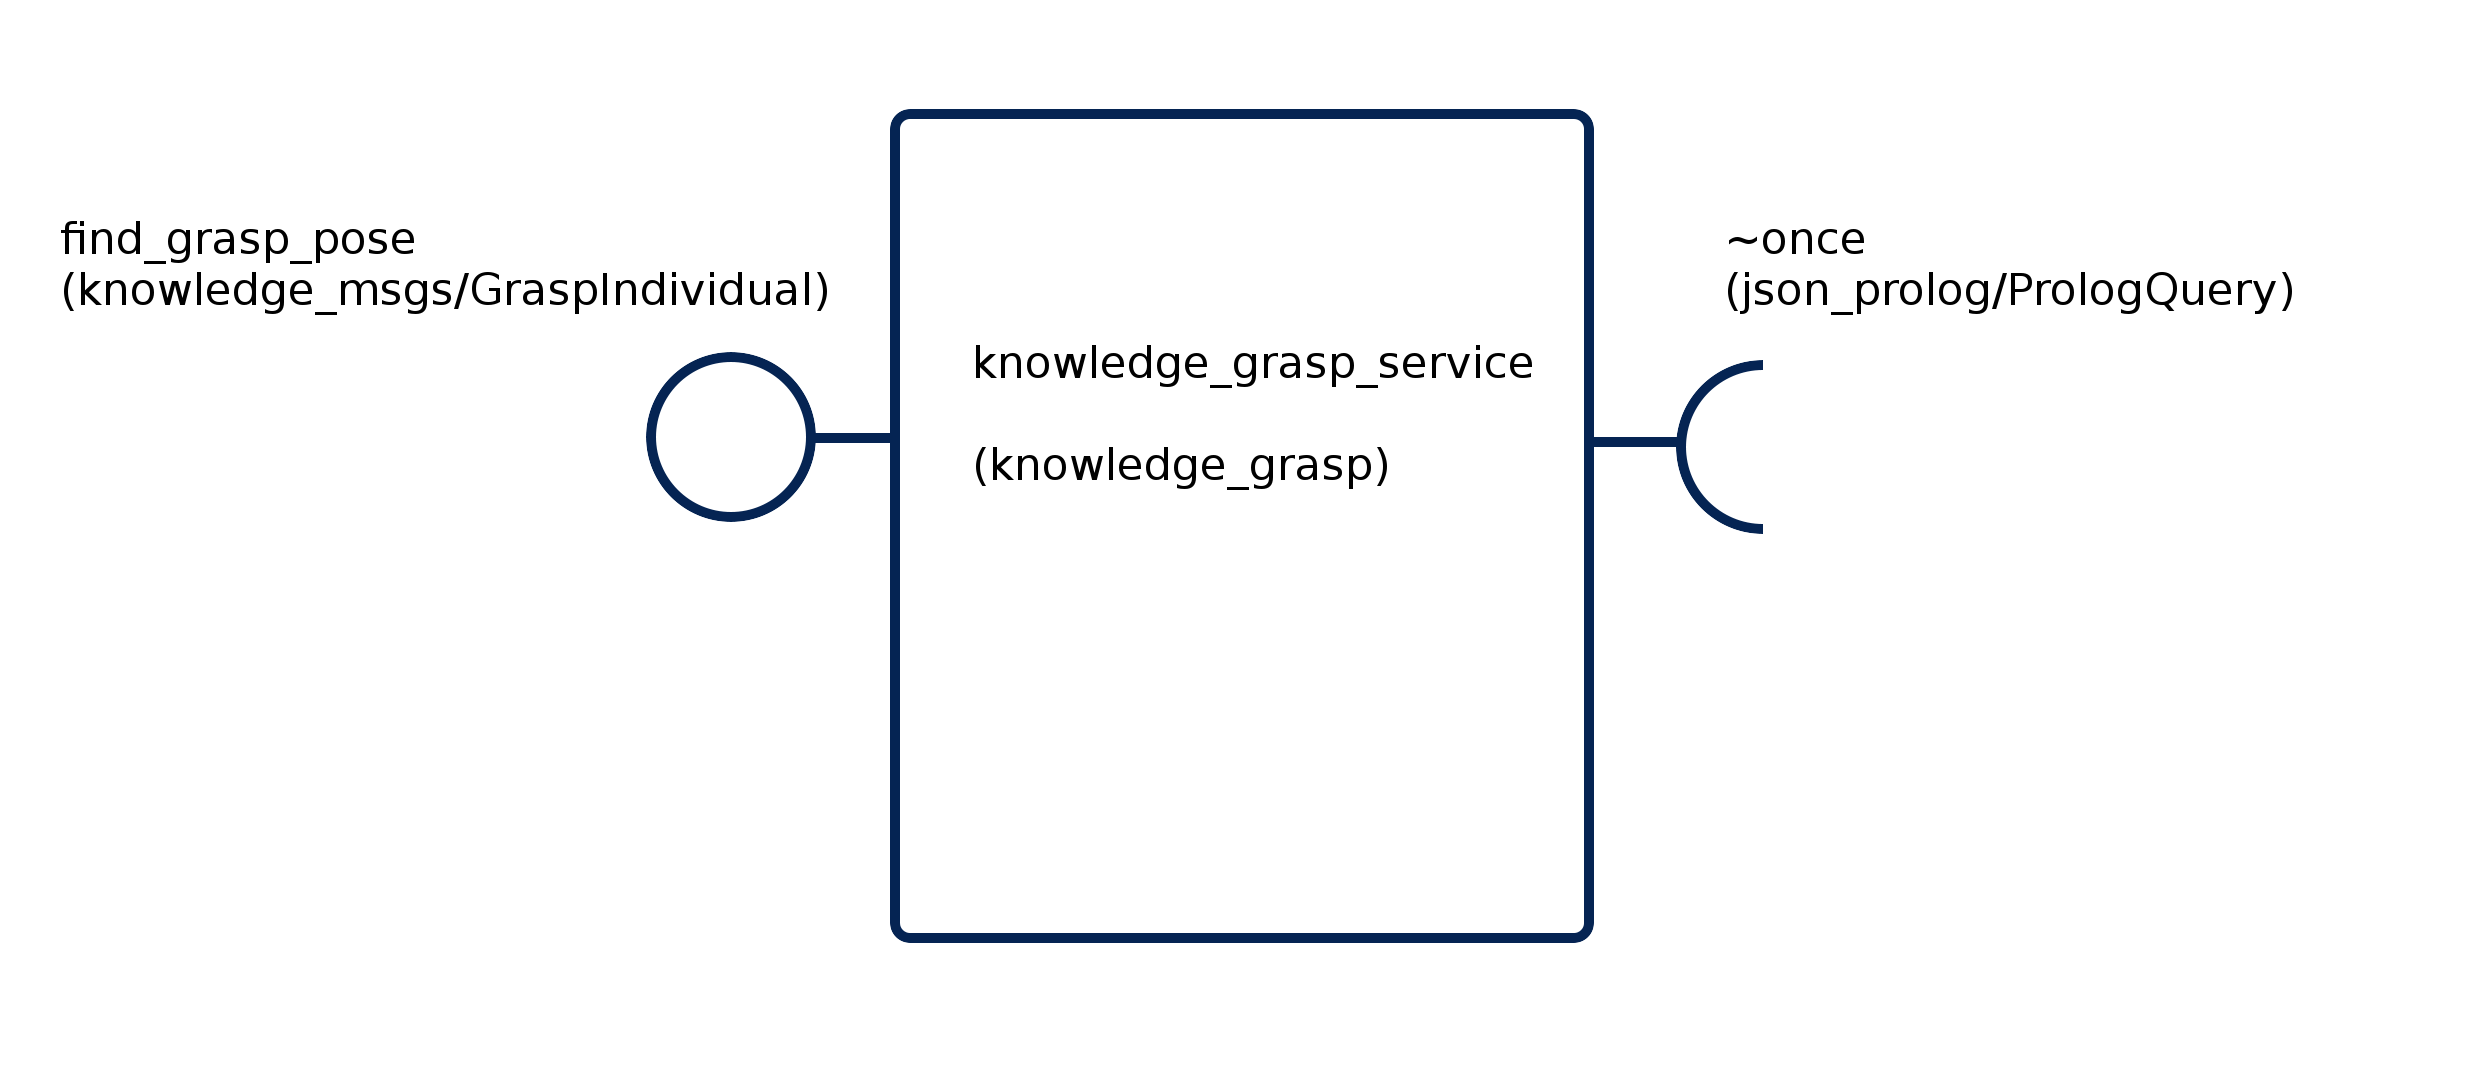
\includegraphics[width=\textwidth]
        {figures/knowledge_grasp_architektur.png}
        \caption{\label{fig:knowledge_grasp_service_node} Architektur der knowledge\_grasp\_service-node}}
\end{figure}
      
\subsection{Beschreibung des Teilsystems}
\chapterauthor{Max-Phillip Bahr}

\subsubsection{find\_grasp\_pose - Prolog}
\begin{spverbatim}
find_grasp_pose(ObjectClassLabel, Position, Quaternion)
@param ObjectClassLabel Das Objektlabel des zu greifenden Objekts 
       (z.B. suturo_object:'JaMilch')
@param Position Position der GraspPose als Prolog Liste (z.B. [0.0, 0.0, 0.0])
@param Quaternion Orientation der GraspPose also Prolog Liste 
       (z.B. [0.0 0.0 0.0 1.0])

Description : Liest zu einem gegebenen Objektlabel eine zugehörige GraspPose aus der Ontologie aus. Es wird bei der eingespeicherten GraspPose von der Translation des Grippers zum Mittelpunkt des Objekts ausgegangen.
\end{spverbatim}

\subsubsection{createQuery - C++}
\begin{spverbatim}
std::string createQuery(std::string object_label)
@param object_label Das Objektlabel.
@return Den aus dem Objektlabel zusammengesetzten Query-String.

Description : Baut aus dem Objektlabel einen Query-String für die Prolog-Methode find_grasp_pose zusammen.
\end{spverbatim}

\subsubsection{find\_grasp\_pose - C++}
\begin{spverbatim}
bool find_grasp_pose(knowledge_msgs::GraspIndividual::Request  &req, 
                             knowledge_msgs::GraspIndividual::Response &res)
@param req Adresse des Request Objekts von GraspIndividual das bearbeitet werden soll.
@param res Adresse zum schreiben des Response Objekts von GraspIndividual.
@return true wenn Methode erfolgreich, false wenn nicht.

Description : Die Methode liest das Objektlabel aus req aus und baut mit createQuery einen QueryString  der mit der once-Methode an den Prolog Server geschickt wird. Wenn Prolog mit find_grasp_pose (Prolog Methode) eine Lösung zur Query findet (also die GraspPose aus der Ontologie ausliest) wird diese in das Response Objekt 
geschrieben und true zurückgegeben. Wenn nicht wird eine Fehlermeldung ausgegeben und false zurückgegeben.
\end{spverbatim}

\section{svm\_classifier}
\chapterauthor{Alexander Haar}
Das svm\_classifier-Paket dient zur Ermittlung eines Objektlabels anhand eines Featurevektors.

\subsection{svm\_classifier}
\begin{figure}[!htb]
        \center{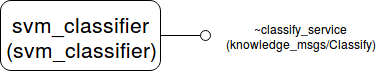
\includegraphics[width= 10cm]
        {figures/svm_classifier.png}
        \caption{\label{fig:classifier} Architektur der svm\_classifier-node}}
\end{figure}

\subsection{svm\_training\_data\_collector}
\begin{figure}[!htb]
        \center{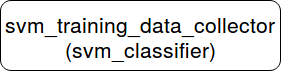
\includegraphics[width= 5cm]
        {figures/svm_training_data_collector.png}
        \caption{\label{fig:training_data} Architektur der svm\_training\_data\_collector-node}}
\end{figure}

\subsection{svm\_trainer}
\begin{figure}[!htb]
        \center{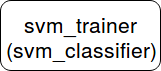
\includegraphics[width=5cm]
        {figures/svm_trainer.png}
        \caption{\label{fig:trainer} Architektur der svm\_trainer-node}}
\end{figure}
      
\subsection{Beschreibung des Teilsystems}
\chapterauthor{Alexander Haar}

\subsubsection{main - Python}
\begin{verbatim}
if __name__ == '__main__'
Beschreibung: Lädt die svm_model.sav Datei und startet den Classify- Service.
\end{verbatim}

\subsubsection{save\_training\_set - Python}
\begin{verbatim}
def save_training_set()
Beschreibung: Nachdem alle Trainingsdaten gesammelt wurden, speichert diese 
Funktion alle Daten als sav- Datei.
\end{verbatim}

\subsubsection{get\_corresponding\_normals\_histogram\_file - Python}
\begin{verbatim}
def get_corresponding_normals_histogram_file(color_histogram_file)
Beschreibung: Findet zu einem Farbhistogramm das entsprechende Normalshistogramm. 
@param color_histogram_file: Das Farbhistogramm.
@return: Das korrespondierende Normalshistogramm.
\end{verbatim}

\subsubsection{get\_features - Python}
\begin{verbatim}
def get_features(label, color_histogram_file)
Beschreibung: Ermittelt anhand des Labels der Klasse und der Farbhistogrammdatei 
den Featurevektor
@param label: Das Label der Klasse.
@param color_histogram_file: Die Farbhistogrammdatei.
@return: Der resultierende Featurevektor.
\end{verbatim}

\subsubsection{collect\_training\_data - Python}
\begin{verbatim}
def collect_training_data()
Beschreibung: Startet das Sammeln von Trainingsdaten.
\end{verbatim}

\subsubsection{main - Python}
\begin{verbatim}
if __name__ == '__main__'
Beschreibung: Initialisiert den Paketpfad und startet das Sammeln 
von Trainingsdaten.
\end{verbatim}

\subsubsection{plot\_confusion\_matrix - Python}
\begin{verbatim}
def plot_confusion_matrix(cm, classes, normalize=False, title='Confusion matrix',
cmap=plt.cm.Blues)
Beschreibung: Erstellt eine Konfusionsmatrix und stellt diese graphisch dar. 
@param cm: Die echten Labels.
@param classes: Die vorhergesagten Labels.
\end{verbatim}

\subsubsection{main - Python}
\begin{verbatim}
if __name__ == '__main__'
Beschreibung: Lädt die Trainingsdaten und startet das Trainieren der SVM, 
welche anschließend gespeichert wird.
\end{verbatim}

\subsection{Schnittstellen}
\chapterauthor{Alexander Haar}

\subsubsection{Service Server classify\_service}
\begin{verbatim}
def classify(req)
Beschreibung: Service- Methode, welche einen Featurevektor klassifiziert.
@param req: Die Anfrage an den Service, welche den Featurevektor enhält.  
@param res: Die Antwort des Services, welche das Label enthält.
\end{verbatim}

\subsection{Programmablauf}
\chapterauthor{Alexander Haar}
\subsubsection{Schritt 1: Trainingsdaten sammeln und speichern}
Es werden aus csv- Dateien die Featurevektoren mit Labels ausgelesen und als sav- Datei gespeichert.

\subsubsection{Schritt 2: Trainieren und speichern einer SVM} 
Die Trainingsdaten werden geladen, danach wird eine SVM mit den Daten trainiert und gespeichert.

\subsubsection{Schritt 3: Laden der SVM und Klassifizieren von Featurevektoren}
Die beiden vorherigen Schritte werden nur einmal im Vorfeld ausgeführt. Das Hauptprogramm lädt die SVM und startet anschließend den Classify- Service.

\section{beliefstate}
\chapterauthor{Alexander Haar}
Das beliefstate-Paket dient dazu sich Aktionen die der Roboter ausgeführt hat zu speichern und auf Anfrage zu ermitteln, welcher Gripper belegt ist und welche Objekte als nächstes weggeräumt werden sollen. Außerdem spawnt der Knoten die Objektkoordinatensysteme und spawnt außerdem das Mesh des Objekts.

\begin{figure}[!htb]
        \center{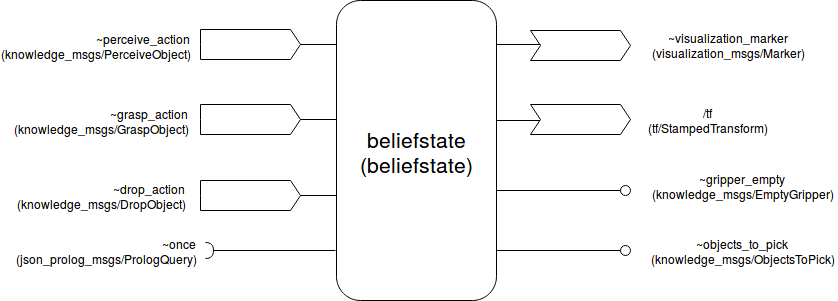
\includegraphics[width=\textwidth]
        {figures/beliefstate.png}
        \caption{\label{fig:beliefstate_node} Architektur der beliefstate-node}}
\end{figure}
      
\subsection{Beschreibung des Teilsystems}
\chapterauthor{Alexander Haar}

\subsubsection{to\_underscore - Python}
\begin{verbatim}
def to_underscore(name)
Beschreibung: Übersetzt einen string von Camelcase- Schreibweise 
in underscore- Schreibweise. 
@param name: Der string in Camelcase- Schreibweise.
@return: Der string in underscore- Schreibweise.
\end{verbatim}

\subsubsection{object\_url\_to\_object\_name - Python}
\begin{verbatim}
def object_url_to_object_name(url)
Beschreibung: Extrahiert aus einer Owl-Url den Namen eines Objekts.
@param url: Die Owl- Url.
@return: Der Objektname.
\end{verbatim}


\subsubsection{prolog\_query\_false - Python}
\begin{verbatim}
def prolog_query_false(query_result)
Beschreibung: Evaluiert, ob eine Prologanfrage zu false auswertet.
@param query_result: Resultat einer einer Prologanfrage.
@return: True, falls die Prologanfrage zu false evaluiert und false sonst.
\end{verbatim}

\subsubsection{prolog\_query\_true - Python}
\begin{verbatim}
def prolog_query_true(query_result)
Beschreibung: Evaluiert, ob eine Prologanfrage zu true auswertet.
@param query_result: Resultat einer einer Prologanfrage.
@return: True, falls die Prologanfrage zu true evaluiert und false sonst.
\end{verbatim}

\subsubsection{point\_to\_prolog\_list - Python}
\begin{verbatim}
def point_to_prolog_list(point)
Beschreibung: Übersetzt einen Punkt in eine Prologliste.
@param point: Der zu übersetzende Punkt.
@return: Die resultierende Prologliste.
\end{verbatim}

\subsubsection{pose\_to\_prolog\_list - Python}
\begin{verbatim}
def pose_to_prolog_list(pose)
Beschreibung: Übersetzt eine Pose in eine Prologliste.
@param pose: Die zu übersetzende Pose.
@return: Die resultierende Prologliste.
\end{verbatim}

\subsubsection{gripper\_as\_string - Python}
\begin{verbatim}
def gripper_as_string(gripper)
Beschreibung: Übersetzt eine Gripperkonstante in einen string.
@param gripper: Die zu übersetzende Gripperkonstante.
@return: Der resultierende string.
\end{verbatim}

\subsubsection{create\_query\_for\_perceive\_object - Python}
\begin{verbatim}
def create_query_for_perceive_object(perceive_object_msg)
Beschreibung: Erzeugt anhand einer PerceiveObject.msg eine Prologanfrage.
@param perceive_object_msg: Die PerceiveObject.msg.
@return: Die resultierende Prologanfrage.
\end{verbatim}

\subsubsection{create\_query\_for\_grasp\_object - Python}
\begin{verbatim}
def create_query_for_grasp_object(grasp_object_msg)
Beschreibung: Erzeugt anhand einer GraspObject.msg eine Prologanfrage.
@param grasp_object_msg: Die GraspObject.msg.
@return: Die resultierende Prologanfrage.
\end{verbatim}

\subsubsection{create\_query\_for\_drop\_object - Python}
\begin{verbatim}
def create_query_for_drop_object(drop_object_msg)
Beschreibung: Erzeugt anhand einer DropObject.msg eine Prologanfrage.
@param drop_object_msg: Die DropObject.msg.
@return: Die resultierende Prologanfrage.
\end{verbatim}

\subsubsection{create\_query\_object\_attached\_to\_gripper - Python}
\begin{verbatim}
def create_query_object_attached_to_gripper(gripper)
Beschreibung: Erzeugt anhand einer Gripperkonstante eine Prologanfrage.
@param gripper: Die Gripperkonstante.
@return: Die resultierende Prologanfrage.
\end{verbatim}

\subsubsection{object\_exists - Python}
\begin{verbatim}
def object_exists(object_class)
Beschreibung: Evaluiert, ob ein Objekt bereits wahrgenommen wurde und in 
der Wissensbasis existiert.
@param object_class: Das zu überprüfende Objekt.
@return: True, falls das Objekt in der Wissensbasis existiert und false sonst.
\end{verbatim}

\subsubsection{pose\_stamped\_to\_position\_tupel - Python}
\begin{verbatim}
def pose_stamped_to_position_tupel(pose_stamped)
Beschreibung: Übersetzt die Position eines PoseStamped in ein Tupel.
@param pose_stamped: Der zu übersetzende PoseStamped.
@return: Das resultierende Tupel.
\end{verbatim}

\subsubsection{pose\_stamped\_to\_quaternion\_tupel - Python}
\begin{verbatim}
def pose_stamped_to_quaternion_tupel(pose_stamped)
Beschreibung: Übersetzt das Quaternion eines PoseStamped in ein Tupel.
@param pose_stamped: Der zu übersetzende PoseStamped.
@return: Das resultierende Tupel.
\end{verbatim}

\subsubsection{quaternion\_to\_prolog\_list - Python}
\begin{verbatim}
def quaternion_to_prolog_list(quaternion)
Beschreibung: Übersetzt ein Quaternion in eine Prologliste.
@param quaternion: Das zu übersetzende Quaternion.
@return: Die resultierende Prologliste.
\end{verbatim}

\subsubsection{spawn\_object\_frame - Python}
\begin{verbatim}
def spawn_object_frame(object_name, object_pose)
Beschreibung: Spawnt an der angegebenen Pose ein Objektkoordinatensystem 
und das entsprechende Mesh.
@param object_name: Der Name des Objekts.
@param object_pose: Die Pose des Objekts.
\end{verbatim}

\subsubsection{update\_object\_frame - Python}
\begin{verbatim}
def update_object_frame(object_name, object_pose)
Beschreibung: Ändert die Pose des angegeben Objekts auf die übergebene.
@param object_name: Der Name des Objekts.
@param object_pose: Die Pose des Objekts.
\end{verbatim}

\subsubsection{change\_reference\_frame - Python}
\begin{verbatim}
def change_reference_frame(object_name, new_reference_frame_id)
Beschreibung: Verändert das Referenzframe des Objektkoordinatensystems 
auf das übergeben Koordinatensystem.
@param object_name: Der Name des Objekts.
@param new_reference_frame_id: Das neu Referenzkoordinatensystem.
\end{verbatim}

\subsubsection{spawn\_object\_mesh - Python}
\begin{verbatim}
def spawn_object_mesh(object_name)
Beschreibung: Spawnt ein Mesh in dem entsprechenden Objektkoordinatensystem.
@param object_name: Der Name des Objekts.
\end{verbatim}

\subsubsection{main - Python}
\begin{verbatim}
__name__ == '__main__
Beschreibung: Startet alle Service- Server und Subscriber die dieser Knoten benötigt.
\end{verbatim}

\subsubsection{object\_exists - Prolog}
\begin{verbatim}
object_exists(ObjectClass)
Beschreibung: Prüft, ob ein Individual dieser Klasse bereits in der
Wissensbasis vorhanden ist
@param ObjectClass: Die zu prüfende Objektklasse.
\end{verbatim}

\subsubsection{process\_perceive\_action - Prolog}
\begin{verbatim}
process_perceive_action(ObjectClass, PoseList, ReferenceFrame)
Beschreibung: Fügt ein Individual der Objektklasse an der angegebenen 
Pose im Referenzframe hinzu.
@param ObjectClass: Die Klasse der hinzuzufügenden Individuals.
@param PoseList: Die Pose des Objekts als Liste.
@param ReferenceFrame: Das Referenzframe.
\end{verbatim}

\subsubsection{process\_grasp\_action - Prolog}
\begin{verbatim}
process_grasp_action(ObjectClass, GripperIndividual)
Beschreibung: Fügt eine GraspAction zur Wissensbasis hinzu unter 
Verwendung des angegeben Grippers und der Objektklasse.
@param ObjectClass: Die Objektklasse.
@param GripperIndividual: Linker oder rechter Gripper.
\end{verbatim}

\subsubsection{process\_drop\_action - Prolog}
\begin{verbatim}
process_drop_action(GripperIndividual)
Beschreibung: Fügt eine DropAction zur Wissensbasis hinzu unter 
Verwendung des angegeben Grippers.
@param GripperIndividual: Linker oder rechter Gripper.
\end{verbatim}

\subsubsection{object\_attached\_to\_gripper - Prolog}
\begin{verbatim}
object_attached_to_gripper(GripperIndividual, ObjectIndividual)
Beschreibung: Prüft, ob sich ein Objekt in dem angegebenen Gripper befindet.
@param GripperIndividual: Linker oder rechter Gripper.
@param ObjectIndividual: Das Objekt, welches sich im Gripper befindet.
\end{verbatim}

\subsubsection{get\_latest\_object\_pose - Prolog}
\begin{verbatim}
get_latest_object_pose(ObjectIndividual, PoseList)
Beschreibung: Gibt die zuletzt bekannte Pose des Objekts zurück.
@param ObjectIndividual: Das Objekt.
@param PoseList: Die Pose des Objekts.
\end{verbatim}

\subsubsection{get\_objects\_on\_kitchen\_island\_counter - Prolog}
\begin{verbatim}
get_objects_on_kitchen_island_counter(ObjectList)
Beschreibung: Gibt eine Liste aller Objekte die noch verteilt
werden müssen zurück.
@param ObjectList: Eine Liste aller Objekte die noch verteilt werden müssen.
\end{verbatim}

\subsubsection{get\_two\_objects\_on\_kitchen\_island\_counter\_with\_same\_storage\_place - Prolog}
\begin{verbatim}
get_two_objects_on_kitchen_island_counter_with_same_storage_place(Object1, Object2)
Beschreibung: Gibt die zwei Objekte zurück, welche als nächstes verteilt werden sollen.
@param Object1: Das erste Objekt.
@param Object2: Das zweite Objekt.
\end{verbatim}

\subsection*{Schnittstellen}
\chapterauthor{Alexander Haar}

\subsubsection*{Subscriber process\_perceive\_action}
\begin{verbatim}
def process_perceive_action(perceive_object_msg)
Beschreibung: Erstellt anhand der Message eine Prologanfrage und
sendet diese an den json_prolog- Server. 
@param perceive_object_msg: Die PerceiveObject.msg
\end{verbatim}

\subsubsection*{Subscriber process\_grasp\_action}
\begin{verbatim}
def process_grasp_action(grasp_object_msg)
Beschreibung: Erstellt anhand der Message eine Prologanfrage und
sendet diese an den json_prolog- Server. 
@param grasp_object_msg: Die GraspObject.msg
\end{verbatim}

\subsubsection*{Subscriber process\_drop\_action}
\begin{verbatim}
def process_drop_action(drop_object_msg)
Beschreibung: Erstellt anhand der Message eine Prologanfrage und
sendet diese an den json_prolog- Server. 
@param drop_object_msg: Die DropObject.msg
\end{verbatim}

\subsubsection*{Service Server gripper\_empty}
\begin{verbatim}
def gripper_empty(req)
Beschreibung: Die Anfrage an den Server ist leer. Zurückgegeben werden
zwei booleans, welche angeben, ob der Gripper belegt ist.
@param req: Die Anfrage an den Service.
@return: Die Antwort des Services.
\end{verbatim}

\subsubsection*{Service Server object\_to\_pick}
\begin{verbatim}
def objects_to_pick(req)
Beschreibung: Gibt die zwei Objekte zurück, welche als nächstes weggeräumt werden sollen.
@param req: Die Anfrage an den Service.
@return: Die Antwort des Services.
\end{verbatim}

\subsection*{Programmablauf}
\chapterauthor{Alexander Haar}
\subsubsection*{Schritt 1: Wahrnehmen mehrerer Objekte}
Es werden mehre Objekte wahrgenommen und deren Label sowie Pose wird dem beliefstate bekannt gemacht.

\subsubsection*{Schritt 2: Welche zwei Objekte sollen weggeräumt werden?}
Nachdem Alle zu verteilenden Objekte bekannt sind, werden möglichst zwei Objekte ausgewählt, welche den gleichen Lagerplatz besitzen.

\subsubsection*{Schritt 3: Greifen eines Objekts}
Das erste der beiden Objekte wird gegriffen.

\subsubsection*{Schritt 4: Greifen eines weiteren Objekts}
Anschließend wird das zweite Objekt gegriffen.

\subsubsection*{Schritt 5: Abstellen des 1. Objekts}
Der Roboter fährt zum entsprechenden Lagerplatz und stellt es dort ab.

\subsubsection*{Schritt 6: Anfrage welcher der Gripper belegt ist}
Nun wird geprüft, ob beide Gripper leer sind, dies ist nicht der Fall.

\subsubsection*{Schritt 7: Abstellen des 2. Objekts}
Der Roboter fährt zum nächsten Lagerplatz und stellt das zweite Objekt dort ab.

\subsubsection*{Schritt 8: Anfrage welcher der Gripper belegt ist}
Erneut wird geprüft, ob beide Gripper leer sind, dies ist jetzt der Fall.

\subsubsection*{Schritt 9: Welche Objekte sollen weggeräumt werden?}
Nun beginnt dieser Prozess wieder bei Schritt 2.


\section{storage\_place}
\chapterauthor{Alexander Haar}
Das storage\_place-Paket dient zur Ermittlung des Lagerplatzes eines Objekts.

\begin{figure}[!htb]
        \center{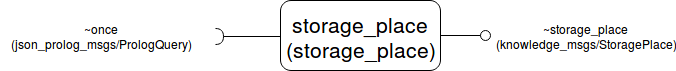
\includegraphics[width=\textwidth]
        {figures/storage_place.png}
        \caption{\label{fig:vision_node} Architektur der storage\_place-node}}
\end{figure}
      
\subsection{Beschreibung des Teilsystems}
\chapterauthor{Alexander Haar}

\subsubsection{createQuery - C++}
\begin{verbatim}
std::string createQuery(std::string object_label)
Beschreibung: Erzeugt eine Prologanfrage, um einen Lagerplatz zu ermitteln.
@param object_label: Der Name des Objekts von dem der Lagerplatz bestimmt werden soll.
\end{verbatim}\label{func:segmentplanes}

\subsubsection{main - C++}
\begin{verbatim}
int main(int argc, char **argv)
Beschreibung: Startet den Knoten.
\end{verbatim}\label{func:findcentergazebo}


\subsubsection{get\_position - Prolog}
\begin{verbatim}
get_position(PositionIndividual, X, Y, Z)
Beschreibung: Extrahiert aus einem Position, die Koordinaten.
@param PositionIndividual: Die Position
@param X: Die X- Koordinate
@param Y: Die Y- Koordinate
@param Z: Die Z- Koordinate
\end{verbatim}\label{func:findposes}

\subsubsection{get\_scale - Prolog}
\begin{verbatim}
get_scale(StorageAreaIndividual, Width, Height)
Beschreibung: Extrahiert aus einer Lagerfläche die Ausmaße.
@param StorageAreaIndividual: Die Lagerfläche
@param Width: Die Breite der Lagerfläche
@param Height: Die Höhe der Lagerfläche
\end{verbatim}\label{func:estimatesurfacenormals}

\subsubsection{storage\_area - Prolog}
\begin{verbatim}
storage_area(ObjectClass, StorageAreaIndividual)
Beschreibung: Ermittelt zu einer Objektklasse die Lagerfläche.
@param ObjectClass: Die Objektklasse zu der eine Lagerfläche ermittelt werden soll.
@param StorageAreaIndividual: Die ermittelte Lagerfläche.
\end{verbatim}\label{func:apply3dfilter}

\subsubsection{storage\_place - Prolog}
\begin{verbatim}
storage_place(ObjectClass, [X, Y, Z], Width, Height)
Beschreibung: Ermittelt zu einer Objektklasse den Lagerplatz.
@param ObjectClass: Die Objektklasse zu der ein Lagerplatz ermittelt werden soll.
@param X: Die X- Koordinate des Lagerplatzes.
@param Y: Die Y- Koordinate des Lagerplatzes.
@param Z: Die Z- Koordinate des Lagerplatzes.
@param Width: Die Breite des Lagerplatzes.
@param Height: Die Höhe des Lagerplatzes.
\end{verbatim}\label{func:estimateplaneindices}

\subsection{Schnittstellen}
\chapterauthor{Alexander Haar}

\subsubsection{Service Server find\_storage\_place}
\begin{verbatim}
bool find_storage_place(knowledge_msgs::StoragePlace::Request &req,
 knowledge_msgs::StoragePlace::Response &res)
Beschreibung: Service- Methode, welche einen Lagerplatz für Objekte ermittelt.
@param req: Die Anfrage an den Service, welche den Namen des Objekts enthält.  
@param res: Die Antwort des Services, welche das Zentrum und die Ausmaße des Lagerplatzes
            enthält.
@return: true, falls der Aufruf erfolgreich war und false sonst.
\end{verbatim}\label{func:findcluster}

\subsection{Programmablauf}
\chapterauthor{Alexander Haar}
\subsubsection{Schritt 1: Anfrage an den Service- Server}
Eine Objektklasse wird an den Service- Server übergeben.
\subsubsection{Schritt 2: Erstellen der Prologanfrage}
Anhand der Objektklasse wird eine Prologanfrage erstellt und an den json\_prolog- Server geschickt.
\subsubsection{Schritt 3: Ermitteln des Lagerplatzes} 
Durch die oben definierten Prologregeln wird unter Verwendung von only- restrictions der Lagerplatz ermittelt.
\subsubsection{Schritt 4: Zurückgeben der Antwort}
Die vom json\_prolog- Server erhaltene Antwort wird entsprechend geparst und zurückgegeben.

\newpage

\section*{Methodendokumentation Gruppe Motion}
\section{Node: main (motion\_suturo\_1718)}
\subsection{Architekturbild}
\chapterauthor{Roman Haak}
\begin{figure}[!htb]
        \center{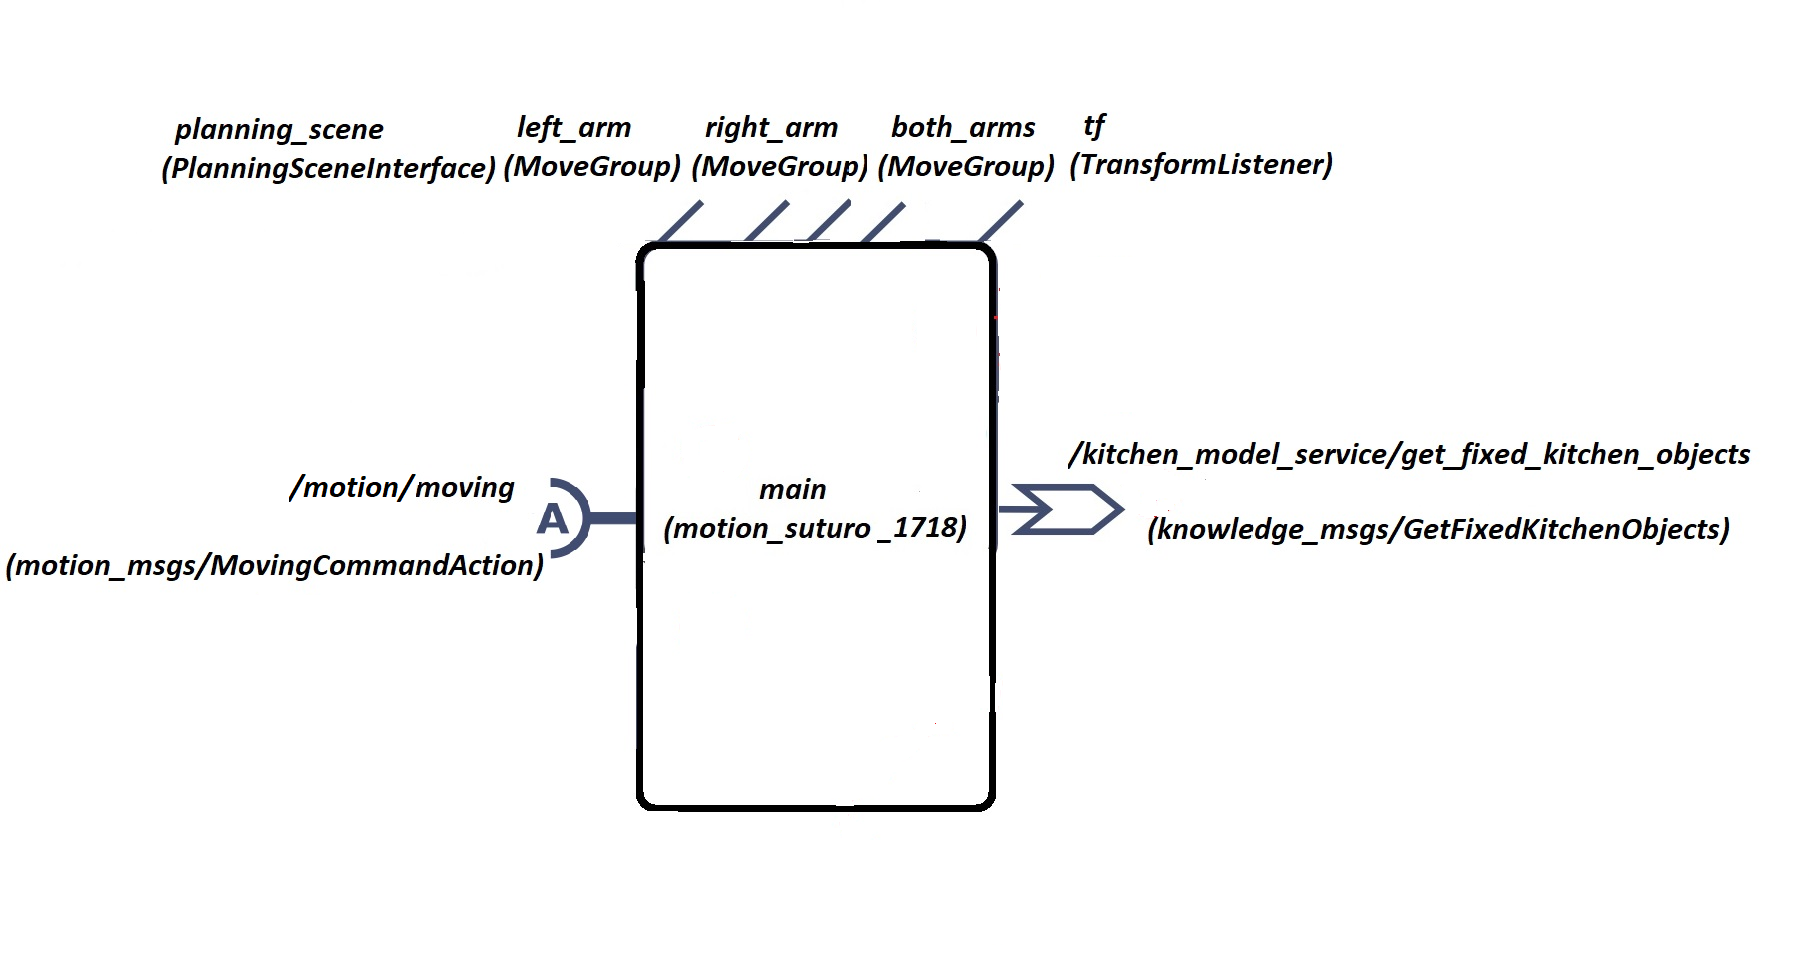
\includegraphics[width=\textwidth]
        {img/Architekturbild.png}
        \caption{\label{fig:motion_node} Architektur der motion-node}}
\end{figure}

\subsection{API}
\subsubsection{Serviceclient}
\chapterauthor{Roman Haak}
'\textit{/kitchen\_model\_service/get\_fixed\_kitchen\_objects}': \\
Dieser Service wird beim Initialisieren unseres Programms aufgerufen. Hierüber werden die Abmessungen der Objekte der IAI-Küche in die \textit{PlanningScene} geladen, damit der Roboter sich nur kollisionsfrei bewegt(siehe \textit{Kapitel 1.2.2}, Abschnitt zur '\textit{planning\_scene}').\\
Die Objekte sind dabei durch eine Höhe, Breite und Länge als \textit{Box-Collider} definiert.


\subsubsection{ActionServer}
\chapterauthor{Maximilian Bertram}
'\textit{/motion/moving}': \\
Vom Typ '\textit{motion\_msgs/MovingCommand}': \\
\begin{lstlisting}[caption={Definition der MovingCommandAction},captionpos=b]
#goal definition
geometry_msgs/PointStamped point_stamped
uint8 command
uint8 UNKNOWN=0
uint8 MOVE_STANDARD_POSE=1
uint8 MOVE_RIGHT_ARM=2
uint8 MOVE_LEFT_ARM=3
---
#result definition
bool successful
---
#feedback definition
#bool finished
\end{lstlisting}

Über die MovingCommand Action ist es möglich Bewegungs-Anweisungen an unseren Actionserver zu senden. Die MovingCommand Action besteht dabei aus folgenden Attributen:
\begin{center}
	\begin{tabular}{ l | l | p{7cm}}
		Name & Type & Bedeutung \\ \hline
		goal\_ point & geometry\_ msgs/PointStamped & Der Endpunkt der Bewegung als PointStamped mit definierter frameid im Header Teil des PointStamped \\ \hline
		command & uint8 & Konstante, die die Art des Befehls definiert (siehe Tabelle weiter unten) \\
	\end{tabular}
\captionof{table}{Felder des Goals der MovingCommandAction}
\end{center}
  
Folgende Konstanten sind für die MovingCommand Action Message definiert:

\begin{center}
	\begin{tabular}{ l | l | p{7cm}}
		Name & Int-Wert & Bedeutung \\ \hline
		UNKNOWN & 0 & - \\ \hline
		MOVE\_ STANDARD\_ POSE & 1 & Roboter Arme in die Initiale Pose bewegen (es wird kein PointStamped in der Message benötigt) \\ \hline
		MOVE\_ RIGHT\_ ARM & 2 & Rechten Arm zu gegebenem PointStamped bewegen \\ \hline
		MOVE\_ LEFT\_ ARM & 3 & Linken Arm zu gegebenem PointStamped bewegen \\
	\end{tabular}
	\captionof{table}{Konstanten der MovingCommandAction}
\end{center}

Folgendes wird zurückgegeben:


\begin{center}
	\begin{tabular}{ l | l | p{10cm}}
		Name & Type & Bedeutung \\ \hline
		successfull & bool & true/false, je nachdem ob die Bewegung erfolgreich durchgeführt werden konnte oder nicht. Im Falle eines Fehlers, werden die MoveIt Error-Codes mit einer entsprechenden Beschreibung auf der Konsole ausgegeben. \\
	\end{tabular}
	\captionof{table}{Rückgabe der MovingCommandAction}
\end{center}


\subsection{Beschreibung des Teilsystems}
\subsubsection{Übersicht}
\chapterauthor{Roman Haak}
Dieser Teil des Systems ist für das Bewegen des PR2 in eine bestimmte Position, bzw. zu einem bestimmten Punkt hin verantwortlich.\\
Zum Ausführen von Bewegungen des PR2 benutzen wir das '\textit{MoveIt-Framework}'. Dieses Framework bietet dabei ein '\textit{MoveGroup-Interface}' an, mit dessen Hilfe es dem Benutzer möglich ist, mit einfachen Funktionsaufrufen Bewegungen auszuführen. Die dahinter steckenden Logiken und Umrechnungen, welche zum letztendlichen Bewegen des Armes nötig sind, werden dann von dem Framework umgesetzt, ohne dass der Benutzer sich darum kümmern muss.\\
Wie wir dieses Framework benutzen, wird im Folgenden vorgestellt.

\subsubsection{Klassenvariablen}
\chapterauthor{Roman Haak}
Im Folgenden werden kurz die wichtigsten Variablen der Klasse '\textit{main}' vorgestellt, um die Funktionsweise des \textit{MoveGroup-Interfaces} zu verdeutlichen:\\\\
\textit{\textbf{planning\_scene}} vom Typ \textit{\textbf{PlanningSceneInterface}}:\\
Über diese Variable ist es uns möglich die sogenannte '\textit{PlanningScene}' des PR2 zu befüllen. Über die \textit{PlanningScene} wird dem PR2 signalisiert, an welcher Stelle sich Objekte befinden, damit Kollisionen mit diesen Vermieden werden können. Wird von dem Benutzer versucht, über das \textit{MoveIt\_Framework} eine Bewegung auszuführen, prüft das Framework zunächst, ob diese Bewegung kollisionsfrei ausgeführt werden kann und bricht mit entsprechender Fehlermeldung ab, falls es in der \textit{PlanningScene} ein Objekt gibt, mit dem der PR2 kollidieren würde. \\
Die Objekte der PlanningScene sind in unserem Fall die Küchenobjekte der IAI-Küche und werden definiert durch einen '\textit{Box-Collider}' mit gewisser Höhe, Breite und Länge.\\\\
\textit{\textbf{both\_arms}}, \textit{\textbf{left\_arm}}, \textit{\textbf{right\_arm}} vom Typ \textit{\textbf{MoveGroupInterface}}:\\
Über Variablen des \textit{MoveGroupInterfaces} können Befehle zum Bewegen eines bestimmten Körperteils abgeschickt werden. Bei uns gibt es dabei drei Gruppen für linken, rechten und beide Arme.\\
So können wir den Endpunkt der jeweiligen kinematischen Kette zu einem bestimmten Punkt hinbewegen oder auch die Gelenkwinkel der Gelenke einer Gruppe einstellen. Das Berechnen einer Trajektorie übernimmt dabei das \textit{MoveIt-Framework}.\\
Es wird von dem \textit{MoveGroup}-Objekt eine entsprechende Rückmeldung in Form eines \textit{MoveItErrorCodes} über den Erfolg der Ausführung gegeben.\\\\
\textit{\textbf{tf}} vom Typ \textit{\textbf{TransformListener}}:\\
Mit Hilfe des \textit{TransformListeners} können Transformationen zwischen Koordinatensystemen zu einem bestimmten Zeitpunkt durchgeführt werden. Das ist in unserem Fall z.B. nötig, wenn der Arm zu einem bestimmten Punkt bewegt werden soll, der aber in einem anderen Koordinatensystem angegeben ist, als unser \textit{MoveGroup}-Objekt zum Planen verwendet.\\


\subsection{Programmablauf}
\chapterauthor{Maximilian Bertram}

Folgendes ist beim starten unserer Node zu beachten:

Es muss bereits der kitchen\_ model\_ export Service von knowledge gestartet sein, damit wir direkt beim starten der Node die PlanningScene richtig befüllen können.

Zum starten unserer Node stehen zwei launch-files zur Verfügung, eins für die Simulation (\textit{motion\_ main\_ start.launch}) und eins für den echten PR2 (\textit{motion\_ main\_ start\_ real\_ pr2.launch}).
\\

'\textit{motion\_ main\_ start.launch}': \\
-Startet leere Simulation (empty world) mit PR2 \\
-Startet MoveIt Move\_ Group (es wird eine für die Simulation des PR2 generierte MoveIt Konfiguration genutzt)\\
-Startet einen static transformer für das Umrechnen von Punkten in der Simulation, da hier die gefakte Lokalisierung/Navigation des PR2 noch nicht funktioniert \\
-Startet unsere Main Node \\

'\textit{motion\_ main\_ start\_ real\_ pr2.launch}': \\
-Startet MoveIt Move\_ Group (es wird die MoveIt Konfiguration des iai\_ pr2 packages genutzt) \\
-Startet unsere Main Node \\
-Ein Static Transformer wird nicht benötigt, da auf dem Roboter die Map von einem Service zur Verfügung gestellt wird \\
-Die Simulation muss auf dem echten PR2 nicht gestartet werden \\

Nach einem erfolgreichen Start, wird der \textit{kitchen\_ model\_ service (siehe Kapitel 1.2.3 - Serviceclient)} aufgerufen und die PlanningScene mit den Objekten der Küche befüllt. \\
Im Falle eines Fehlers beendet sich der Node und es wird eine entsprechende Meldung auf der Konsole ausgegeben. \\
War das Befüllen der PlanningScene erfolgreich wartet der ActionServer auf weitere Befehle in Form von \textit{MovingCommandAction-Messages}.
Wird eine neue MovingCommandAction-Message gesendet, wird das \textit{Command} der Message geparst und die entsprechende Gruppe (\textit{linker Arm, rechter Arm, beide Arme}) bewegt. \\
Es wird der Punkt (falls erforderlich) in das entsprechende Koordinatensystem der zu bewegenden Gruppe umgerechnet. Anschließend wird mit MoveIt ein entsprechender Bewegungsplan erstellt.\\ 
Wenn ein entsprechender Bewegungsplan existiert und die Gruppe an den Punkt ohne Kollision mit der PlanningScene bewegt werden kann, wird die Bewegung ausgeführt und \textit{true} zurückgegeben.
Existiert kein Bewegungsplan (z.B.: Gruppe kann rein technisch nicht an den Punkt gelangen) oder  wenn es keine Möglichkeit gibt an den Punkt ohne Kollision zu gelangen, wird \textit{false} zurückgegeben und der entsprechende MoveItErrorCode mit Beschreibung auf der Konsole ausgegeben und keine Bewegung durchgeführt. \\





%UNTERSCHIED LAUNCHFILE FÜR SIMULATION UND ECHTER ROBOTER -> LADEN DER KONFIGURATIONSDATEIEN - SIMULATION ODER ECHTER ROBOTER
%STARTEN DER NAVIGATIONSSACHEN -> AUCH HIER UNTERSCHIED SIMULATION UND ECHTER ROBOTER
%INITIALISIEREN DER KÜCHE, WARTEN AUF CALL DES ACTIONSERVERS, AUSFÜHREN (FALLS MÖGLICH), RÜCKMELDUNG AN ACTIONCLIENTS (IN SIMULATION UND ECHT GLEICH)
\subsubsection{Besonderheiten/Besondere Algorithmen}
\chapterauthor{Maximilian Bertram}

\textbf{VisualizationMarker}

Wenn der linke/rechte Arm bewegt wird, werden dabei 2 VisualizationMarker gepublished, welche in RViz angezeigt werden können. Im Idealfall befinden sich diese beiden Punkte exakt an der gleichen Position. Der gelbe Marker zeigt den gewünschten Endpunkt der Bewegung vor dem umrechnen, der rote Marker zeigt den Punkt nach dem Umwandeln in das Koordinatensystem der zu bewegenden Gruppe.

%ÜBERHAUPT VORHANDEN? PARSEN DER MOVEITERRORCODES? VISUALIZATION-MARKER? ORIENTATION DES GRIPPERS?

\newpage

\section*{Methodendokumentation Gruppe Vision}

\section{Vision}
\subsection{Vorwort Vision}
\chapterauthor{Alexander Link}
Da einige Teile der Dokumentation überarbeitet und nicht komplett neu geschrieben wurden, ist zu beachten, dass die Autoren der Vision-Teile zu der Dokumentation von Meilenstein 1 genau umgekehrt waren. Auch ist hinzuzufügen, dass an vielen Funktionen Tammo Wübbena und Alexander Link zugleich beteiligt waren. In solchen Fällen sind beide Autoren mit "Beide"\ abgekürzt.

\subsection{Überblick Vision}
\chapterauthor{Alexander Link}
Das Vision-Paket \footnote{im weiteren Verlauf auch Vision-Package, vision-node oder einfach Paket oder vision genannt} dient zur Akquirierung und Verarbeitung visueller Informationen durch die Kinect-Kamera des PR2-Roboters.

\begin{figure}[!htb]
        \center{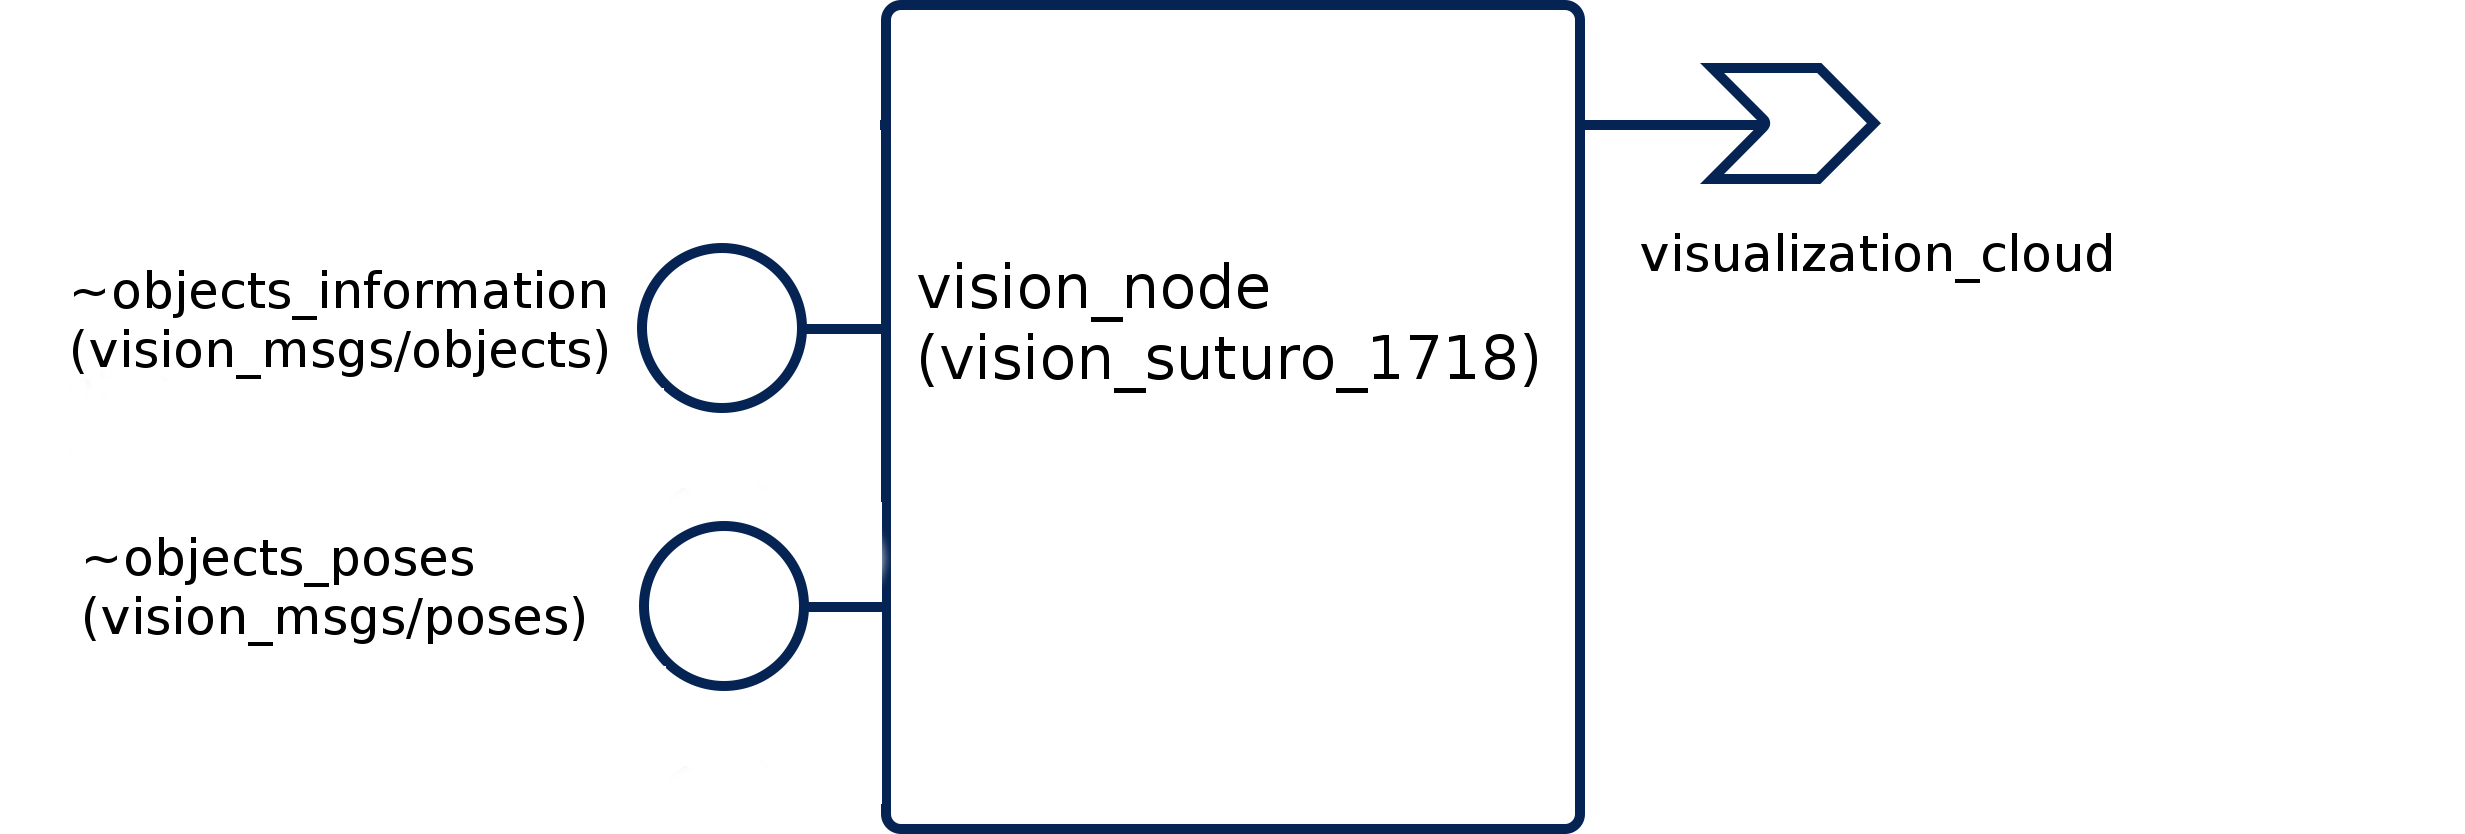
\includegraphics[width=\textwidth]
        {figures/vision_diagram_milestone_2.png}
        \caption{\label{fig:vision_node} Architektur der vision-node}}
\end{figure}
      
\subsection{Beschreibung des Teilsystems}
\chapterauthor{Tammo Wübbena, Update: Alexander Link}

\subsubsection{Abkürzungen durch short\_types.h}
\chapterauthor{Alexander Link (Doku), Beide (Code)}
Für bessere Lesbarkeit haben wir typedef Kürzel verwendet:
\begin{verbatim}
typedef pcl::PointCloud<pcl::PointXYZ>::Ptr PointCloudXYZPtr;
typedef pcl::PointCloud<pcl::PointXYZRGB>::Ptr PointCloudRGBPtr;
typedef pcl::PointCloud<pcl::Normal>::Ptr PointCloudNormalPtr;
typedef pcl::PointCloud<pcl::PointNormal>::Ptr PointCloudPointNormalPtr;
typedef pcl::PointCloud<pcl::PointXYZ> PointCloudXYZ;
typedef pcl::PointCloud<pcl::PointXYZRGB> PointCloudRGB;
typedef pcl::PointCloud<pcl::Normal> PointCloudNormal;
typedef pcl::PointIndices::Ptr PointIndices;
typedef std::vector<pcl::PointIndices> PointIndicesVector;
typedef std::vector<pcl::PointIndices::Ptr> PointIndicesVectorPtr;

typedef geometry_msgs::PointStamped PointStamped;
typedef pcl::PointCloud<pcl::VFHSignature308>::Ptr PointCloudVFHS308Ptr;
typedef sensor_msgs::PointCloud2 SMSGSPointCloud2;
typedef std::vector<pcl::PointCloud<pcl::PointXYZ>::Ptr> PointCloudXYZPtrVector;
\end{verbatim}

\subsubsection*{Perception}

\subsubsection{preprocessCloud}
\chapterauthor{Alexander Link (Doku), Tammo Wübbena (Code)}
\begin{verbatim}
findCluster(const PointCloudXYZPtr kinect)
Beschreibung: Wendet unsere Filter auf eine Punktwolke an.
@param: kinect Punktwolke
@return: Vorprozessierte Punktwolke
\end{verbatim}\label{func:preprocesscloud}

\subsubsection{segmentPlanes}
\chapterauthor{Alexander Link (Doku), Beide (Code)}
\begin{verbatim}
void segmentPlanes(PointCloudRGBPtr cloud_cluster)
Beschreibung: Segmentiert Flächen, die nicht für die gesuchten Objekte
relevant sind.
@param: PointCloud, aus der Flächen entfernt werden sollen.
\end{verbatim}\label{func:segmentplanes}

\subsubsection{findCluster}
\chapterauthor{Alexander Link (Doku), Beide (Code)}
\begin{verbatim}
std::vector<PointCloudRGBPtr> findCluster(PointCloudRGBPtr kinect)
Beschreibung: Findet die Objekte und gibt eine Punktwolke pro Objekt zurück.
@param: Punktwolke der Kinect
@return: Punktwolken der Objekte
\end{verbatim}\label{func:findcluster}

\subsubsection{findCenterGazebo}
\chapterauthor{Alexander Link (Doku), Beide (Code)}
\begin{verbatim}
geometry_msgs::PointStamped findCenterGazebo()
Beschreibung: Gibt einen künstlichen Punkt zurück (Den Mittelpunkt des
Modells, 
das an Gazebo übergeben wurde).
@return: Künstlicher 3D-Mittelpunkt
\end{verbatim}\label{func:findcentergazebo}


\subsubsection{findPoses}
\chapterauthor{Alexander Link (Doku), Beide (Code)}
\begin{verbatim}
std::vector<geometry_msgs::PoseStamped> 
findPoses(const std::vector<PointCloudRGBPtr> clouds_in)
Beschreibung: Errechnet Position und Rotation der Objekte in den übergebenen
Punktwolken.
@param: Punktwolken der Objekte
@return: Posen der Objekte
\end{verbatim}\label{func:findposes}

\subsubsection{estimateSurfaceNormals}
\chapterauthor{Alexander Link (Doku), Beide (Code)}
\begin{verbatim}
PointCloudNormalPtr estimateSurfaceNormals(PointCloudRGBPtr input)
Beschreibung: Schätzt die Normalen einer Punktwolke.
@param: Punktwolke, zu der die Normalen berechnet werden sollen
@return: Normalen der übergebenen Punktwolke
\end{verbatim}\label{func:estimatesurfacenormals}

\subsubsection{apply3DFilter}
\chapterauthor{Alexander Link (Doku), Beide (Code)}
\begin{verbatim}
PointCloudRGBPtr apply3DFilter(PointCloudRGBPtr input, float x, float y, 
float z)
Beschreibung: Filtert eine Punktwolke, indem sie nur die Punkte in einem
bestimmten Bereich ((-x,x), (-y,y), (0.0,z)) erhält.
@param: Punktwolke, die gefiltert werden soll
		x,y,z Bereiche der Achsen für den Filter
@return Gefilterte Punktwolke
\end{verbatim}\label{func:apply3dfilter}

\subsubsection{estimatePlaneIndices}
\chapterauthor{Alexander Link (Doku), Beide (Code)}
\begin{verbatim}
PointIndices estimatePlaneIndices(PointCloudRGBPtr input)
Beschreibung: Errechnet die Indizes einer Fläche einer Punktwolke.
@param: Punktwolke, dessen Fläche ermittelt werden soll
@return Indizes der Fläche, wenn eine gefunden wurde
\end{verbatim}\label{func:estimateplaneindices}

\subsubsection{extractCluster}
\chapterauthor{Alexander Link (Doku), Beide (Code)}
\begin{verbatim}
PointCloudRGBPtr extractCluster(PointCloudRGBPtr input, PointIndices indices, 
bool negative);
Beschreibung: Extrahiert Objekt-Cluster anhand übergebener Punktwolke und
Indizes.
@param: input Punktwolke, aus der ein Cluster extrahiert werden soll
		indices Indizes der Punkte in input, die extrahiert werden sollen
		negative Entscheidet, ob Indizes extrahiert werden sollen (false) oder
		alle Punkte, außer den in Indizes angegebenen (true).
@return Objekt-Cluster Punktwolke
\end{verbatim}\label{func:extractcluster}

\subsubsection{mlsFilter}
\chapterauthor{Alexander Link (Doku), Beide (Code)}
\begin{verbatim}
PointCloudRGBPtr mlsFilter(PointCloudXYZPtr input);
Beschreibung: Glättet Punktwolke unter Verwendung eines Moving-Least-Squares
Algorithmus.
@param: Punktwolke, die mittels MLS-Algorithmus geglättet wird
@return Geglättete Punktwolke
\end{verbatim}\label{func:mlsfilter}

\subsubsection{voxelGridFilter}
\chapterauthor{Alexander Link (Doku), Beide (Code)}
\begin{verbatim}
PointCloudRGBPtr voxelGridFilter(PointCloudRGBPtr input)
Beschreibung: Filtert eine Punktwolke mit dem Voxel-Gitter-Filter.
@param: Zu filternde Punktwolke
@return Mit einem Voxel-Gitter gefilterterte (und damit gedownsamplete)
Punktwolke
\end{verbatim}\label{func:voxelgridfilter}

\subsubsection{outlierRemoval}
\chapterauthor{Alexander Link (Doku), Beide (Code)}
\begin{verbatim}
PointCloudRGBPtr outlierRemoval(PointCloudRGBPtr input)
Beschreibung: Entfernt Punkte aus Punktwolke, die als zu weit außen liegend
(outlier) oder als Rauschen erkannt werden.
@param: Punktwolke, die von Rauschen befreit werden soll
@return Gefilterte Punktwolke
\end{verbatim}\label{func:outlierremoval}

\subsubsection{cvfhRecognition}
\chapterauthor{Alexander Link (Doku + Code)}
\begin{verbatim}
PointCloudVFHS308Ptr cvfhRecognition(PointCloudRGBPtr input)
Beschreibung: Errechnet features eines Objekts in einer Punktwolke als
VFHSignature308
@param: Punktwolke, dessen features berechnet werden sollen
@return Features als VFHSignature308
\end{verbatim}\label{func:cvfhRecognition}

\subsubsection{euclideanClusterExtraction}
\chapterauthor{Alexander Link (Doku + Code)}
\begin{verbatim}
std::vector<PointCloudRGBPtr> euclideanClusterExtraction(PointCloudRGBPtr
input)
Beschreibung: Trennt cluster einer Punktwolke voneinander.
@param: Punktwolke
@return Eine Punktwolke pro cluster/Objekt
\end{verbatim}\label{func:euclideanClusterExtraction}

\subsubsection{SACInitialAlignment}
\chapterauthor{Alexander Link (Doku), Tammo Wübbena (Code)}
\begin{verbatim}
PointCloudRGBPtr SACInitialAlignment(std::vector<PointCloudRGBPtr> objects,
                                std::vector<PointCloudVFHS308Ptr> features,
                                PointCloudRGBPtr target)
Beschreibung: Errechnet Ausrichtung von Objekten bezüglich Zielen per sample
consensus
@param: objects Punktwolken, features als VFHSignature308, target PointCloud
@return Punktwolke
\end{verbatim}\label{func:sacinitialalignment}

\subsubsection{iterativeClosestPoint}
\chapterauthor{Alexander Link (Doku), Tammo Wübbena (Code)}
\begin{verbatim}
PointCloudRGBPtr iterativeClosestPoint(PointCloudRGBPtr input,
                                       PointCloudRGBPtr target)
Beschreibung: Errechnet Ausrichtung eines Objekts zu einem Ziel anhand eines
iterativen 
			  Closest-Point-Algorithmus.
@param: input Punktwolke, target Punktwolke
@return Punktwolke
\end{verbatim}\label{func:iterativeClosestPoint}

\subsubsection{produceColorHist}
\chapterauthor{Alexander Link (Doku), Tammo Wübbena (Code)}
\begin{verbatim}
std::vector<uint64_t> produceColorHist
(pcl::PointCloud<pcl::PointXYZRGB>::Ptr  cloud)
Beschreibung: Errechnet ein Farbhistogramm einer Punktwolke.
@param: input Punktwolke eines Objekts, dessen Farbhistogramm errechnet werden
soll
@return Farbhistogramm als floats (r,g,b)
\end{verbatim}\label{func:produceColorHist}

\subsubsection{getAllFeatures}
\chapterauthor{Alexander Link (Doku), Tammo Wübbena (Code)}
\begin{verbatim}
void getAllFeatures(std::vector<PointCloudRGBPtr> all_clusters,
                    std::vector<float> vfhs_vector,
                    std::vector<uint64_t> color_features_vector)
Beschreibung: Errechnet CVFH- und Farb-features für alle übergebenen Objekte.
@param: Punktwolken der Objekte, deren features errechnet werden sollen
\end{verbatim}\label{func:getallfeatures}

\subsubsection{getCVFHFeatures}
\chapterauthor{Alexander Link (Doku), Tammo Wübbena (Code)}
\begin{verbatim}
void getCVFHFeatures(std::vector<PointCloudRGBPtr> all_clusters,
std::vector<float> current_features_vector)
Beschreibung: Errechnet CVFH-features von Punktwolken
@param: Punktwolken der Objekte, deren CVFH-features errechnet werden sollen
@return: CVFH features (Histogramme der Winkel zwischen einer zentralen
viewpoint direction und jeder Normalen
\end{verbatim}\label{func:getcvfhfeatures}

\subsubsection{getColorFeatures}
\chapterauthor{Alexander Link (Doku), Tammo Wübbena (Code)}
\begin{verbatim}
void getColorFeatures(std::vector<PointCloudRGBPtr> all_clusters,
std::vector<uint64_t> color_features_vector)
Beschreibung: Errechnet Farbfeatures von Punktwolken
@param: Punktwolken der Objekte, deren Farbfeatures errechnet werden sollen
	    Vektor für Farbfeatures, der befüllt wird
\end{verbatim}\label{func:getcolorfeatures}

\subsubsection{getTargetByLabel}
\chapterauthor{Alexander Link (Doku), Tammo Wübbena (Code)}
\begin{verbatim}
PointCloudRGBPtr getTargetByLabel(std::string label)
Beschreibung: Lädt die PCD-Datei des Objekts, das zum übergebenen label
gehört.
@param: String label
@return Objekt-Punktwolke aus der jeweiligen PCD-Datei
\end{verbatim}\label{func:gettargetbylabel}


\subsection*{vision\_node}
\chapterauthor{Alexander Link (Doku), Beide (Code)}
\subsubsection{sub\_kinect\_callback}
\begin{verbatim}
void sub_kinect_callback(PointCloudRGBPtr kinect)
Beschreibung: Callback-Funktion für das kinect topic. Speichert die PointCloud
ab, sodass sie bereitsteht, wenn sie zur Prozessierung benötigt wird.
@param: Punktwolke des kinects
\end{verbatim}\label{func:subkinectcallback}
\subsubsection{start\_node}
\begin{verbatim}
void start_node(int argc, char **argv)
Beschreibung: Startet die Node zur Prozessierung von Punktwolken und der
Kommunikation mit anderen Nodes.
@param: argc und argv ungenutzt
\end{verbatim}\label{func:startnode}
\subsubsection{getObjects}
\begin{verbatim}
bool getObjects(	vision_suturo_msgs::objects::Request &req, 
			    vision_suturo_msgs::objects::Response &res)
Beschreibung: Service zum Extrahieren von Objekten und deren Informationen aus
einer Szene.
@param: req leere request, res Antwort mit den extrahierten Objekten nach
ObjectsInfo.msg
@return true wenn service call erfolgreich, ansonsten false
\end{verbatim}\label{func:getobjects}


\subsection*{CloudTransformer}
\chapterauthor{Alexander Link (Doku + Code)}

\subsubsection{extractAbovePlane}
\begin{verbatim}
PointCloudRGBPtr CloudTransformer::extractAbovePlane(PointCloudRGBPtr input)
Beschreibung: Findet die Hauptfläche (-> Tischplatte) und extrahiert nur die
Punkte über dieser Fläche.
@param: Punktwolke
@return Extrahierte Punktwolke (ohne die Hauptfläche)
\end{verbatim}\label{func:extractaboveplane}
\subsubsection{transform}
\begin{verbatim}
PointCloudRGBPtr CloudTransformer::transform(const PointCloudRGBPtr cloud,
std::string target_frame,
                 std::string source_frame)
Beschreibung: Transformiert eine Punktwolke in einen anderen frame.
@param: cloud Punktwolke, target_frame, source_frame
@return Transformierte Punktwolke
\end{verbatim}\label{func:transform}

\subsection*{saving}
\chapterauthor{Alexander Link (Doku), Beide (Code)}
Hilfsfunktionen zum Speichern von Punktwolken als .PCD-Dateien.

\begin{verbatim}
void savePointCloudRGBNamed(pcl::PointCloud<pcl::PointXYZRGB>::Ptr cloud,
                            std::string filename);
                            
void savePointCloudXYZ(pcl::PointCloud<pcl::PointXYZ>::Ptr cloud);

void savePointCloudXYZNamed(pcl::PointCloud<pcl::PointXYZ>::Ptr cloud,
std::string filename);

void savePointCloudNormal(pcl::PointCloud<pcl::Normal>::Ptr cloud);

void savePointCloudPointNormal(pcl::PointCloud<pcl::PointNormal>::Ptr cloud);

void savePointCloud(pcl::PointCloud<pcl::PointXYZ>::Ptr objects,
                    pcl::PointCloud<pcl::PointXYZ>::Ptr kinect,
                    pcl::PointCloud<pcl::Normal>::Ptr normals);
\end{verbatim}

\subsection*{viewer}
\chapterauthor{Alexander Link (Doku), Tammo Wübbena (Code)}
Hilfsfunktionen zur Darstellung von Punktwolken.
Enthält auch den momentan ungenutzten Visualization Marker.

\begin{verbatim}
void visualizePointCloud(pcl::PointCloud<pcl::PointXYZ> cloud);

void visualizeNormals(pcl::PointCloud<pcl::PointXYZ>::Ptr cloud,
pcl::PointCloud<pcl::Normal>::ConstPtrnormals);

visualization_msgs::Marker publishVisualizationMarker
(geometry_msgs::PointStamped point);
\end{verbatim}


\subsection{Schnittstellen}
\chapterauthor{Tammo Wübbena}

\subsubsection{Service Server /vision\_suturo/objects\_information}
\begin{verbatim}
objects.srv
@request: -
@response: ObjectsInfo msg (
							normal_features (VHFSignature308 as array)
							color_features (Color Histogram as array)
							object_amount (Number of objects in scene)
							object_information (additional information)
							object_errors (errors while extracting)
							)
\end{verbatim}
Gibt Anzahl, Features von den in einer Szene erkannten Objekten (Clustern) zurück. Die Pose wird für diesen Meilenstein noch nicht ermittelt. Der Service kann weitere Informationen und bei Problemen unterschiedliche Fehlermeldungen zurückgeben.
\\ \\
Die \textit{normal\_features} vom Typ VFHSignature308 und \textit{color\_features} (acht bins) aller Objekte werden konkateniert in Arrays festgehalten. 
Da die Länge der Features für ein Objekt immer gleich ist, kann durch die Anzahl der erkannten Objekte die Länge insgesamt ermittelt werden.

\subsubsection{Service Server /vision\_suturo/objects\_poses}
\begin{verbatim}
poses.srv
@request: string, uint8 (label of classified (recognized) object and its number in the array given by the ObjectsInfo.msg)
@response: ObjectsInfo msg (
							poses (the pose of the requested object)
							)
\end{verbatim}
Nachdem der Service objects\_information aufgerufen wurde, werden die dadurch erzeugten Features von Planning (Weiterleitung) und Knowledge (Klassifizierung) bearbeitet. Die erkannten Objekte werden dann von Knowledge jeweils mit einem Label versehen. Der Index wird von Planning bestimmt (durch teilen des übergebenen Feature-Arrays). Danach werden die Objekte von unserem Paket bearbeitet und die Pose durch Vergleich mit den jeweiligen Meshes ermittelt. Danach werden die Posen zurück an Planning übergeben.

\subsubsection{Subscriber REAL\_KINECT\_POINTS\_FRAME}
\begin{verbatim}
@response: PointCloudRGBPtr kinect
\end{verbatim}
Gibt eine Punktwolke unseres Sichtfelds (Szene oder Scene) zurück. Dabei wird auf das Topic \textit{/kinect\_head/depth\_registered/points} horcht. Alternativ kann mit \textit{SIM\_KINECT\_POINTS\_FRAME} auf \textit{/head\_mount\_kinect/depth\_registered/points} auf Simulationsdaten gehorcht werden.
\\ \\
Die Callback-Funktion wird im loop immer wieder aufgerufen, solange die Node noch aktiv ist bzw. der roscore-server besteht.

\subsection{Programmablauf}
\chapterauthor{Tammo Wübbena}
\subsubsection{Schritt 1: Erkennen der Punktwolke}
Ein Subscriber empfängt die zu verarbeitenden Punktwolken des Kinect-Sensors und hält die wahrgenommene Szene aktuell.
\subsubsection{Schritt 2: Service-Aufruf \textit{/vision\_suturo/objects\_information}}
Jedes mal, wenn der Service \textit{/vision\_suturo/objects\_information} durch Planning aufgerufen wird, wird die Funktion \textit{findCluster} in perception.h ausgeführt. 
\subsubsection{Schritt 3: Vorbereiten auf die Extraktion} 
In \textit{findCluster} wird die Punktwolke zunächst folgendermaßen vorbearbeitet:

\begin{itemize} 
\item Ein PassThrough Filter, der den Sichtbereich begrenzt.
\item Ein VoxelGrid Filter zum Downsampling der eingehenden Punktwolke, indem für viele kleine 3-dimensionale Boxen der Mittelpunkte aller enthaltenden Punkte berechnet wird.
\item Ein MovingLeastSquares Filter, der Flächen begradigt, um Ungenauigkeiten der Daten vorzubeugen.
\item Das Entfernen von Flächen, die zu groß sind, um zum gesuchten Objekt gehören zu können. Dies passiert mehrmals, wenn es mehrere solcher Flächen im Sichtfeld gibt.
\end{itemize}
Eine Outlier-Removal wird nicht mehr benötigt, da die folgende Euclidean Cluster Extraction ''Ausreißer'', also weit von den Clustern entfernte Punkte nicht extrahiert.\\
\subsubsection{Schritt 3b: Ausweichen auf Simulationsdaten}
Sollte es zu irgendeinem Zeitpunkt beim Filtern oder der Segmentierung zu Problemen kommen, weil beispielsweise die resultierende Punktwolke leer ist, wird auf die direkten Daten des Zielobjekts aus gazebo ausgewichen, wenn möglich.
\\
\subsubsection{Schritt 4: Cluster Extraktion}
Mit \textit{EuclideanClusterExtracion} werden die nun segmentierten Objekte (alle noch in einer Punktwolke zusammengefasst) extrahiert und in einzelne Cluster gespeichert.
\\
\subsubsection{Schritt 5: Berechnen von Features und Posen}
Es werden die Normal-Features, Color-Features für die Klassifikation durch Knowledge und die Posen der einzelnen Objekte berechnet.
 
\subsubsection{Schritt 6: Befüllen der MSG}
Die einzelnen Features und Posen (letzteres aktuell noch nicht getestet) werden in der Message (ObjectsInfo.msg) gespeichert und zur weiteren Bearbeitung an Planning weitergegeben.

\subsubsection{Schritt 7: Ermitteln der Pose}
Die von Knowledge gelabelten Objekte werden mit ihren jeweiligen Meshes abgeglichen und durch SACInitialAlignment werden ihre jeweiligen Posen ermittelt.

\subsection*{Visualization-Publisher}
Der Visualization-Publisher ''publiziert'' (advertise) die extrahierten Cluster als zusammenhängende Punktwolke

\newpage
\section{Nutzungsbeschreibung}

\subsection{Installation und Ausführung von Planning}

\subsubsection{Installation}
\chapterauthor{Vanessa Hassouna}
\begin{itemize}


\item[a] Laufen alle anderen Systeme (Vision,Knowledge und Motion), muss für Planning folgendes Repository hinzufügt werden: \url{https://github.com/menanuni/planning_suturo_1718.git}. 

\item[b] Ist die Arbeitsumgebung vollständig gebaut, wird CRAM installiert \url{http://cram-system.org/installation}.

\item[c] Nun wird die Entwicklungsumgebung installiert mit: \textbf{sudo apt-get install emacs}. Achtung: Bei der Verwendung von Ubuntu 14.04 muss der neueste Lisp 'compiler' noch hinzugefügt werden \url{https://sourceforge.net/projects/sbcl/files/sbcl/1.3.1/
} (meistens x86-64 Version). Diese Datei entpacken und im Terminal (im richtigen Ordner) den Befehl: \textbf{sh install.sh} eingeben.
\end{itemize}

\subsubsection{Ausführung}
\chapterauthor{Vanessa Hassouna}
\begin{itemize}

\item Zuerst muss im Terminal \textbf{roslisp\_repl} eingegeben werden, daraufhin startet emacs. 

\item Nun wird in der Repl (dort wo cl-user steht) ein "\textbf{,}" (ausgesprochen Komma) eingegeben.

\item Nun wird \textbf{r-l-s} eingegeben und mit \textbf{ENTER} bestätigt. Es folgt die Eingabe des Namens für ein Paket: \textbf{planning\_main\_programm} wird mit zweimaligem Befehl \textbf{ENTER} bestätigt.

\item Zum Schluss wird noch in dem cl-user Fenster \textbf{(planning-main-programm::main)} eingegeben und mit \textbf{ENTER} bestätigt (die Klammern gehören auch dazu).
\end{itemize}


\subsection{Installation und Ausführung von Motion}

\subsubsection{Installation}
\chapterauthor{RH, MB}
\begin{itemize}


\item[a] Zunächst müssen folgende Repositories in den source-Ordner des Workspaces hinzugefügt werden:  \\
\url{https://github.com/menanuni/motion_suturo_1718} \\
\url{https://github.com/menanuni/msgs_suturo_1718} \\
\url{https://github.com/menanuni/knowledge_suturo_1718} \\

\item[b] Es muss das MoveIt Framework installiert werden, dazu im Terminal: \\
\textit{sudo apt-get update} \\
\textit{sudo apt-get install ros-indigo-moveit} \\
\textit{echo  \grqq{}source /opt/ros/indigo/setup.bash\grqq{} \textgreater\textgreater \textasciitilde{ }/.bashrc} \\

\item[c] Jetzt kann das System über \textit{catkin build} gebaut werden.

\end{itemize}

\subsubsection{Ausführung}
\chapterauthor{Roman Haak}
\begin{itemize}

\item Zunächst muss über den Befehl \textit{roslaunch kitchen\_model\_export knowledge\_export\_service.launch} ein Teilsystem von \textit{Knowledge} gestartet werden.

\item Anschließend kann unser Knoten über \textit{roslaunch motion motion\_main\_start.launch} gestartet werden, falls er im Kontext einer Simulation ausgeführt werden soll, bzw. \textit{roslaunch motion motion\_main\_start\_real\_pr2.launch}, falls der Knoten auf dem PR2 ausgeführt werden soll.

\item Dann können Befehle an den Actionserver unseres Knotens über das Topic \textit{/moving/goal} abgesetzt werden. Zur Erläuterung des Actionservers siehe Dokumentation der Gruppe \textit{motion}.
\end{itemize}


\subsection{Installation und Ausführung von Vision}

\subsubsection{Installation (mit gazebo)}
\chapterauthor{Alexander Link}

\textbf{Voraussetzungen}

\begin{itemize}
\item Ubuntu 14.04
\item ROS Indigo
\item Catkin tools
\item Gazebo 2.2.x
\end{itemize}

\textbf{.bashrc}

Folgendes muss zur .bashrc (oder zshrc) hinzugefügt werden:
\begin{itemize}
\item \textit{export KINECT1=true}
\item \textit{export GAZEBO\_MODEL\_PATH= \$HOME/catkin\_ws/vision\_suturo\_1718/vision/models}
\item \textit{export GAZEBO\_RESOURCE\_PATH= \$HOME/catkin\_ws/vision\_suturo\_1718/vision/worlds}
\end{itemize}

\textbf{Setup}

\begin{itemize}
\item gazebo installieren: \textit{sudo apt-get install ros-indigo-pr2-simulator}

\item Sollten Probleme auftreten, könnte dies durch ein Update von gazebo auf v2.2.6 gelöst werden:
\\
\textit{sudo sh -c 'echo "deb http://packages.osrfoundation.org/gazebo/ubuntu trusty main" > /etc/apt/sources.list.d/gazebo-latest.list'}
\\
\textit{wget http://packages.osrfoundation.org/gazebo.key -O - | sudo apt-key add -}
\\
\textit{sudo apt-get update}

\item Folgende Pakete in den src-Ordner eines catkin workspaces klonen:\\
        \textbf{vision\_suturo\_1718} (this package) \\
        \textbf{msgs\_suturo\_1718}
\item Erst "\textit{catkin build object\_detection}" nutzen, um die messages zu bauen.
\item Dann "\textit{catkin build}" benutzen, um alles andere zu bauen.

\end{itemize}

\textbf{Kinect benutzen}
\begin{itemize}
\item \textit{sudo apt install ros-indigo-freenect-launch freenect libfreenect-bin}
\item \textit{roslaunch freenect\_launch freenect-registered-xyzrgb.launch}
\item (Optional) \textit{roslaunch vision vision\_kinect.launch}
\end{itemize}

\textbf{Dateien speichern}

    \textit{rosrun pcl\_ros pointcloud\_to\_pcd input:=/camera/depth\_registered/point}


\subsubsection{Ausf\"uhrung}
\chapterauthor{Alexander Link}

\textbf{vision\_suturo/objects\_information}
\begin{itemize}
\item Benutzt objects.srv
\item Nimmt keine Argumente.
\item Gibt ObjectsInfo.msg zurück
\begin{itemize}
\item float32[] CVFH-Features
\item uint64[] Farb-Features
\item uint8 Objektmenge
\item string[] Weitere Objektinformationen
\item string[] Fehlermeldung (wenn vorhanden)
\end{itemize}
\end{itemize}
\textbf{vision\_suturo/objects\_poses}
\begin{itemize}
\item Benutzt poses.srv
\item Nimmt ein Label (string) und einen Index (int) entgegen.
\item Gibt einen geometry\_msgs/PoseStamped zurück.
\end{itemize}

\textbf{rosservice}

Unsere Services k\"onnen auch manuell abgerufen werden: \\

\textit{rosservice call vision\_suturo/objects\_information} \\

oder \\

\textit{rosservice call vision\_suturo/objects\_poses}

\subsection{Installation und Ausführung von Knowledge}

\subsubsection{Installation}
\chapterauthor{Alexander Haar}

\begin{itemize}
\item[1.] Java8 installieren:$ https://wiki.ubuntuusers.de/Java/Installation/Oracle_Java/Java_8/ $Wichtig JDK
\item[2.] Repo clonen und bauen
\item[3.] Die folgenden Schritte ausführen: $http://knowrob.org/installation/workspace$
\end{itemize}

\subsubsection{Ausführung}
\chapterauthor{Alexander Haar}

Um alle wichtigen Knoten zu starten muss einfach der Befehl \textit{roslaunch knowledge knowledge\_main.launch} ausgeführt werden. Es wird eine json\_prolog- Node, der PokePositon-Service und der GetFixedKitchenModel- Service gestartet.


\end{document}

